% !TEX root = ../main.tex
% ============================================================================
% CAPÍTULO 4 — IMPLEMENTACIÓN Y PRUEBAS
% ----------------------------------------------------------------------------
% NOTAS DE USO (borrar este bloque antes de la entrega final):
%   1. Este archivo asume \usepackage{booktabs} y \usepackage{graphicx} en el
%      preámbulo del documento principal. Si tu main.tex no los tiene, agrégalos.
%   2. Todo texto entre corchetes [COMPLETAR: ...] debe reemplazarse con tus
%      datos reales una vez realizadas las pruebas. Las tablas de resultados
%      contienen valores de EJEMPLO (marcados como tal) solo para mostrar el
%      formato; no son datos reales y no deben citarse como si lo fueran.
%   3. Los bloques de figura son marcadores de posición (cajas grises). Cuando
%      tengas la fotografía o gráfica, reemplaza el contenido del \fbox por
%      \includegraphics[width=0.8\textwidth]{ruta/imagen.png}.
%   4. Numeración: al usar \chapter, las tablas y figuras se numerarán como
%      4.1, 4.2, etc. automáticamente (asumiendo que este es el capítulo 4).
%   5. Las citas usan \citep{} (estilo natbib/apalike), coherente con el resto
%      de tu tesis. Las entradas .bib están en referencias_cap4.bib adjunto.
%   6. Redacción en tono impersonal/pasivo y en tiempo presente o pretérito,
%      sin primera persona ni futuro, siguiendo los criterios de estilo que
%      ya identificaste para el tribunal (separador decimal con coma, sin
%      "etc.", uso reducido de "el cual/la cual").
% ============================================================================

\chapter{IMPLEMENTACIÓN Y PRUEBAS}

Este capítulo describe el proceso de implementación física del sistema de monitoreo de consumo de combustible, desde el prototipado en protoboard hasta pruebas con la placa de circuito impreso (PCB) definitiva, y expone la metodología experimental empleada para validar su desempeño en condiciones reales de operación. La validación se realiza sobre dos vehículos de características distintas y se contrasta contra un adaptador ELM327 combinado con una aplicación comercial de cálculo de consumo. Esta comparación permite evaluar tanto la exactitud del método de estimación como la fiabilidad del sistema desarrollado frente a una alternativa disponible en el mercado.

\section{Montaje del sistema}

El montaje del sistema se organiza en dos etapas complementarias. En la primera, se ensambla un prototipo funcional sobre protoboard que permite verificar la viabilidad eléctrica y de firmware de la arquitectura propuesta antes de comprometer recursos en la fabricación de la PCB. En la segunda etapa, una vez validado el prototipo, se envía el diseño definitivo a fabricación bajo el proceso de JLCPCB. Este orden de trabajo reduce el riesgo de errores de diseño irreversibles en la placa final y permite depurar el firmware con mayor libertad de modificación del cableado.

\subsection{Prototipado en protoboard}

El prototipo se construye alrededor de la placa de desarrollo ESP32-S3-DevKitC-1 (módulo ESP32-S3-WROOM-1, variante N16R8), que integra el controlador CAN nativo TWAI, evitando así la necesidad del controlador externo MCP2515 empleado en la arquitectura inicial del proyecto. La Tabla~\ref{tab:componentes_protoboard} resume los componentes utilizados en esta etapa.



Siguiendo el proceso de armado:

\begin{itemize}
	\item Colocar primeramente el ESP32-S3 en una ubicación fácil de programar y de alimentar por su puerto de comunicación.
	\item Colocar estratégicamente el SN65HDV230 junto con el OLED, ya que estos componentes comparten una alimentación de 3.3~V.
	\item Después para no arruinar un micro SD se usa un adaptador SD, el cual soldaremos para una mejor conexión al protoboard.
	\item Y como ultimo se conecta una configuración de 4 leds para ayudar la visualización de los periféricos.
	
\end{itemize}

\begin{table}[H]
	\centering
	\captionsetup{labelformat=simple, labelsep=newline, textfont=it, labelfont=bf, justification=raggedright, singlelinecheck=false}
	\caption{Componentes empleados en el prototipo sobre protoboard}
	\label{tab:componentes_protoboard}
	\begin{tabularx}{\textwidth}{>{\raggedright\arraybackslash}p{4.5cm} X >{\centering\arraybackslash}p{2cm}}
		\toprule
		\rowcolor[rgb]{0.851, 0.851, 0.851}
		Componente & Función en el prototipo & Cantidad \\
		\midrule
		ESP32-S3-DevKitC-1 (N16R8) & Unidad de procesamiento principal, TWAI nativo & 1 \\
		Módulo transceptor SN65HVD230 & Adaptación de niveles para el bus CAN & 1 \\
		Módulo lector de tarjeta MicroSD (SPI) & Registro local de datos & 1 \\
		Pantalla OLED SSD1306 (I2C) & Visualización de parámetros en tiempo real & 1 \\
		Módulo regulador step-down 12\,V a 5\,V & Alimentación desde el conector OBD-II & 1 \\
		Conector OBD-II tipo A con cable & Interfaz física con el vehículo & 1 \\
		Protoboard, cables jumper macho-macho y macho-hembra & Interconexión temporal de los módulos & Variable \\
		\bottomrule
	\end{tabularx}
	\vspace{2mm}
	\\
	\begin{minipage}{\linewidth}
		\small 
		
		\textit{Nota.} Relación de elementos de hardware integrados para el montaje preliminar y validación de comunicaciones del sistema.
	\end{minipage}
\end{table}

La Figura~\ref{fig:prototipo} muestra la disposición física del prototipo, referenciada a lo largo de esta sección.

\begin{figure}[H]
	\centering
	\caption{Componentes del prototipo y elementos principales del sistema.}
	\label{fig:prototipo}
	
	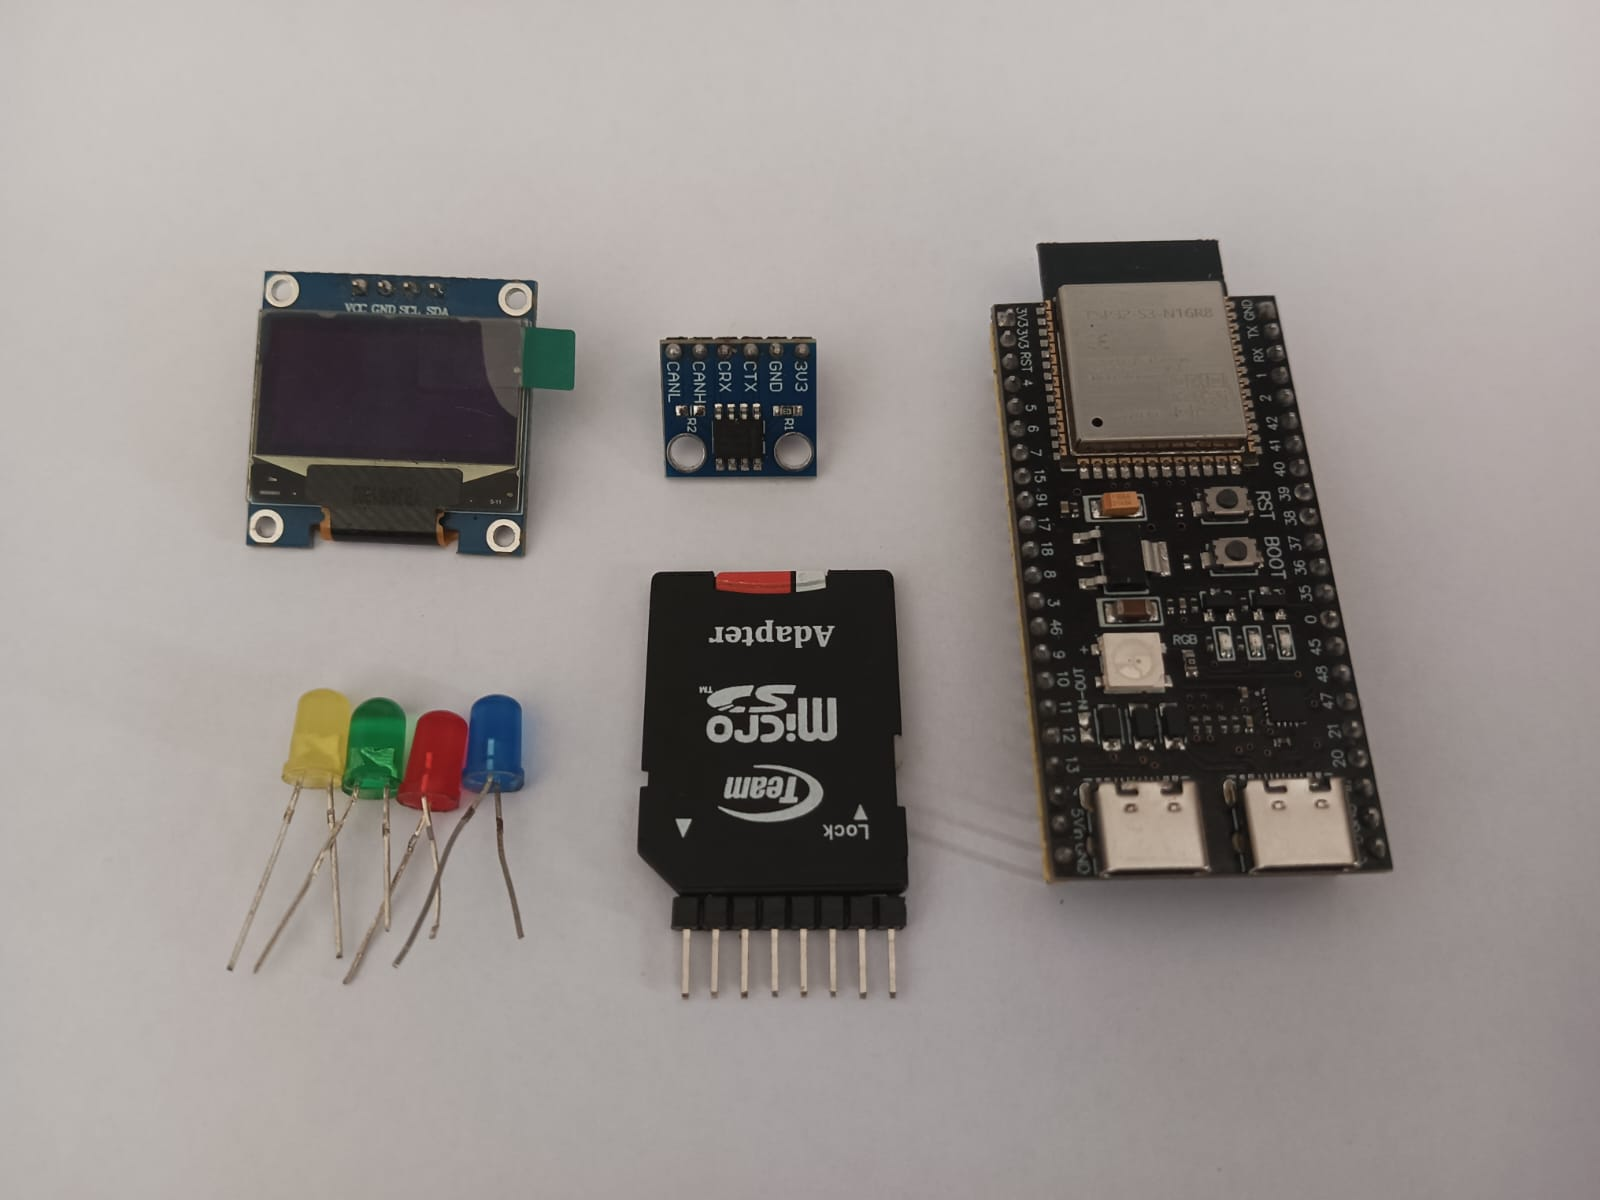
\includegraphics[width=0.8\textwidth]{Images/compo.jpeg}
	\\
	\vspace{2pt}
	{\footnotesize\textit{Nota.} Esquema detallado del patillaje y la comunicación serie entre el microcontrolador principal y los periféricos del sistema. Elaboración propia.}
	
\end{figure}



\subsection{Integración del módulo ESP32-S3 y periféricos en protoboard}

La asignación de pines para el prototipo se resume en la Tabla~\ref{tab:asignacion_pines}. Tal como se presentó en el esquemático de conexión dentro de la sección de diseño de software, esta misma distribución se mantiene para el prototipado físico (Tabla~\ref{tab:mapa_pines}).

\begin{table}[H]
	\centering
	\captionsetup{labelformat=simple, labelsep=newline, textfont=it, labelfont=bf, justification=raggedright, singlelinecheck=false}
	\caption{Asignación de pines GPIO del ESP32-S3 en el prototipo}
	\label{tab:asignacion_pines}
	\begin{tabularx}{\textwidth}{>{\raggedright\arraybackslash}p{4cm} >{\raggedright\arraybackslash}p{4cm} X}
		\toprule
		\rowcolor[rgb]{0.851, 0.851, 0.851}
		Periférico & Pines GPIO & Observaciones \\
		\midrule
		Bus CAN (TWAI) & TX: GPIO4, RX: GPIO5 & Modo listen-only durante pruebas comparativas \\
		Bus I2C (pantalla OLED) & SDA: GPIO8, SCL: GPIO9 & Dirección I2C del controlador SSD1306 \\
		Bus SPI (MicroSD) & MOSI/MISO/SCK/CS: GPIO11-GPIO14 & Sistema de archivos FAT32 \\
		Control de load switches (TPS22918DBVR) & GPIO6,GPIO10 & Habilitación activa en alto (HIGH) \\
		UART de programación & TXD0/RXD0 & Uso exclusivo durante flasheo y depuración \\
		\bottomrule
	\end{tabularx}
	\vspace{2mm}
	\\
	\begin{minipage}{\linewidth}
		\small
		\textit{Nota.} Mapeo de la distribución física de señales digitales y buses de comunicación configurados en el microcontrolador principal.
	\end{minipage}
\end{table}



\begin{figure}[H]
	\centering
	\caption{Diagrama de interconexión de periféricos en el prototipo}
	\label{fig:diagrama_perifericos}
	\begin{tikzpicture}
		
		% Imagen original
		\node[inner sep=0pt] (foto) {
			
\includegraphics[width=0.85\textwidth]{images/prototipo.jpg}
		};
		
		% ------------------------------------------------
		% ESP32
		% ------------------------------------------------
		\node[
		draw=red,
		very thick,
		rounded corners=3pt,
		fill=white,
		align=center,
		font=\bfseries,
		minimum width=2.5cm,
		minimum height=0.8cm
		] (esp32) at ([xshift=-1.0cm,yshift=-0.8cm]foto.north east)
		{ESP32};
		
		\draw[
		->,
		red,
		very thick
		]
		(esp32.west)
		-- ([xshift=-6.3cm,yshift=-4.3cm]foto.north east);
		
		% ------------------------------------------------
		% LEDs
		% ------------------------------------------------
		\node[
		draw=green!60!black,
		very thick,
		rounded corners=3pt,
		fill=white,
		align=center,
		font=\bfseries,
		minimum width=2.5cm,
		minimum height=0.8cm
		] (leds) at ([xshift=0.8cm,yshift=-0.8cm]foto.north west)
		{LEDs};
		
		\draw[
		->,
		green!60!black,
		very thick
		]
		(leds.east)
		-- ([xshift=6.8cm,yshift=-0.8cm]foto.north west);
		
		% ------------------------------------------------
		% OLED
		% ------------------------------------------------
		\node[
		draw=blue,
		very thick,
		rounded corners=3pt,
		fill=white,
		align=center,
		font=\bfseries,
		minimum width=2.5cm,
		minimum height=0.8cm
		] (oled) at ([xshift=0.8cm,yshift=-3.8cm]foto.north west)
		{OLED};
		
		\draw[
		->,
		blue,
		very thick
		]
		(oled.east)
		-- ([xshift=2.8cm,yshift=-6.3cm]foto.north west);
		
		% ------------------------------------------------
		% Tarjeta SD
		% ------------------------------------------------
		\node[
		draw=orange!80!black,
		very thick,
		rounded corners=3pt,
		fill=white,
		align=center,
		font=\bfseries,
		minimum width=2.8cm,
		minimum height=0.8cm
		] (sd) at ([xshift=-1.0cm,yshift=0.8cm]foto.south east)
		{Tarjeta SD};
		
		\draw[
		->,
		orange!80!black,
		very thick
		]
		(sd.west)
		-- ([xshift=-3.0cm,yshift=3.5cm]foto.south east);
		
		% ------------------------------------------------
		% SN65HVD230
		% ------------------------------------------------
		\node[
		draw=violet,
		very thick,
		rounded corners=3pt,
		fill=white,
		align=center,
		font=\bfseries,
		minimum width=3.5cm,
		minimum height=0.8cm
		] (can) at ([xshift=0cm,yshift=0.8cm]foto.south)
		{SN65HVD230};
		
		\draw[
		->,
		violet,
		very thick
		]
		(can.north)
		-- ([xshift=0cm,yshift=2.3cm]foto.south);
		
	\end{tikzpicture}
	\vspace{2pt}
	\\
	{\footnotesize\textit{Nota.} Vista general del prototipo con etiquetas identificativas para cada módulo interactivo. Elaboración propia.}
	
\end{figure}

La integración se verifica de manera incremental: primero se confirma la comunicación I2C con la pantalla OLED mediante un barrido de direcciones (\textit{I2C scanner}), luego se valida la escritura y lectura en la tarjeta MicroSD, y finalmente se habilita el controlador TWAI para la recepción de tramas CAN, como se detalla en la Figura~\ref{fig:diagrama_perifericos}.

\subsection{Placa preliminar en EasyEDA}
\label{sec:placa_preliminar}

Una vez concluidas las pruebas de campo sobre el prototipo en protoboard, se diseñó en EasyEDA una placa preliminar que replica el mismo circuito funcional ya validado (mismo módulo ESP32-S3, mismo transceptor CAN, misma pantalla OLED y microSD), con el único fin de contar con una versión más robusta y cómoda de manejar que las conexiones sueltas de una protoboard, previa a la placa final documentada en el Capítulo~3 (diseñada en Altium Designer). A diferencia de esa placa final, la preliminar resuelve la alimentación con un regulador lineal simple en vez de la conversión conmutada de dos rieles, suficiente para las pruebas de campo dado que no corre con la misma restricción de autonomía en reposo; el esquemático completo, la simulación 3D y las fotografías de la placa fabricada se presentan en el Capítulo~3 (Sección~\ref{sec:pcb_preliminar_diseno}). La fabricación de esta placa preliminar se encargó a Robokit (La Paz) por 150\,Bs (Tabla~\ref{tab:costo_pcb_preliminar}, Capítulo~5), y el ensamblaje de los componentes se realizó manualmente. Al tratarse del mismo circuito ya probado, esta placa no requirió una nueva ronda de pruebas de campo: su función es exclusivamente de robustez física y comodidad de manejo, no de validación técnica adicional sobre lo ya reportado en este capítulo.

\subsection{Conexión al bus CAN del vehículo}

La conexión física al vehículo se realiza a través del conector estandarizado de 16 pines J1962, cuya asignación depende del protocolo de comunicación soportado; desde 2008 la práctica totalidad de los vehículos livianos emplea el protocolo ISO 15765 sobre bus CAN \citep{iso15765}. La Tabla~\ref{tab:pinout_obd} resume los pines relevantes para este proyecto.

\begin{table}[H]
	\centering
	\captionsetup{labelformat=simple, labelsep=newline, textfont=it, labelfont=bf, justification=raggedright, singlelinecheck=false}
	\caption{Pines relevantes del conector OBD-II (J1962) utilizados en el proyecto}
	\label{tab:pinout_obd}
	\begin{tabularx}{\textwidth}{>{\centering\arraybackslash}p{1.5cm} >{\raggedright\arraybackslash}p{4cm} X}
		\toprule
		\rowcolor[rgb]{0.851, 0.851, 0.851}
		Pin & Señal & Uso en el sistema \\
		\midrule
		6 & CAN High (CAN\_H) & Línea diferencial positiva del bus CAN \\
		14 & CAN Low (CAN\_L) & Línea diferencial negativa del bus CAN \\
		16 & Alimentación +12\,V & Entrada al regulador TPS54302DDCR \\
		4 y 5 & Tierra (chasis y señal) & Referencia común del sistema \\
		\bottomrule
	\end{tabularx}
	\vspace{2mm}
	\\
	\begin{minipage}{\linewidth}
		\small
		\textit{Nota.} Identificación de las líneas físicas de alimentación y comunicación del estándar J1962 requeridas para la interfaz con el vehículo.
	\end{minipage}
\end{table}

Con el fin de evitar que el sistema propio introduzca tramas de solicitud adicionales que puedan interferir con el adaptador comercial, el controlador TWAI del ESP32-S3 se configura en modo de solo escucha (\textit{listen-only}), de manera que únicamente recibe y decodifica las tramas sin transmitir reconocimientos ni solicitudes propias. En la Figura \ref{fig:conexion_can}

\begin{figure}[htbp]
	\centering
	\caption{Conexión del sistema propuesto mediante OBD-II}
	\label{fig:conexion_can}
	\begin{tikzpicture}
		
		% Imagen original
		\node[inner sep=0pt] (foto) {
			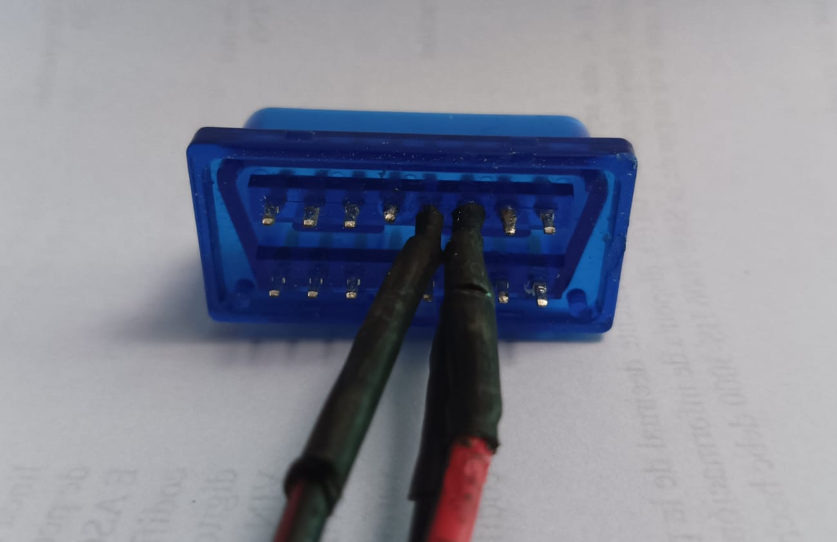
\includegraphics[width=0.7\textwidth]{Images/OBD.png}
		};
		
		% ------------------------------------------------
		% GND (Pin 5) - Arriba Izquierda
		% ------------------------------------------------
		\node[
		draw=blue,
		very thick,
		rounded corners=3pt,
		fill=white,
		align=center,
		font=\bfseries,
		minimum width=2.5cm,
		minimum height=0.8cm
		] (gnd) at ([xshift=-0.5cm,yshift=-0.8cm]foto.north west)
		{GND (Pin 5)};
		
		\draw[
		->,
		blue,
		very thick
		]
		(gnd.east)
		-- ([xshift=5.5cm,yshift=-2.5cm]foto.north west);
		
		% ------------------------------------------------
		% CAN_H (Pin 6) - Arriba Derecha
		% ------------------------------------------------
		\node[
		draw=red,
		very thick,
		rounded corners=3pt,
		fill=white,
		align=center,
		font=\bfseries,
		minimum width=2.5cm,
		minimum height=0.8cm
		] (canh) at ([xshift=0.5cm,yshift=-0.8cm]foto.north east)
		{CAN\_H (Pin 6)};
		
		\draw[
		->,
		red,
		very thick
		]
		(canh.west)
		-- ([xshift=-4.8cm,yshift=-2.9cm]foto.north east);
		
		% ------------------------------------------------
		% CAN_L (Pin 14) - Abajo Derecha
		% ------------------------------------------------
		\node[
		draw=green!60!black,
		very thick,
		rounded corners=3pt,
		fill=white,
		align=center,
		font=\bfseries,
		minimum width=2.5cm,
		minimum height=0.8cm
		] (canl) at ([xshift=0.5cm,yshift=-3.5cm]foto.north east)
		{CAN\_L (Pin 14)};
		
		\draw[
		->,
		green!60!black,
		very thick
		]
		(canl.west)
		-- ([xshift=-4.8cm,yshift=-3.8cm]foto.north east);
		
	\end{tikzpicture}
	\\
	\vspace{2pt}
	{\footnotesize\textit{Nota.} Fotografía de la interfaz OBD-II del vehículo mostrando la derivación del bus CAN. Elaboración propia.}

\end{figure}


\subsection{Instalación física en el vehículo de pruebas}

Buscamos para hacer las pruebas en campo , primero ubicar el puerto OBD2 del vehiculo el cual se ecuentra casi siempre abajo del volante arriba de los pedales, algunos a primera vista otros hay que desarmar unas piezas para llegar a su ubicacion.

En la Figura \ref{fig:instalacion_vehiculo} mostramos la ubicacion de uno de los vehiculos a ponerlo a prueba el cual se desarmo una parte para acceder este se encontro junto alos fusibles de los tableros.

\begin{figure}[H]
	\centering
	\caption{Identificación física del OBD2 en el vehículo antes de las pruebas}
	\label{fig:instalacion_vehiculo}
	\begin{tikzpicture}
		
		% Imagen original
		\node[inner sep=0pt] (foto) {
			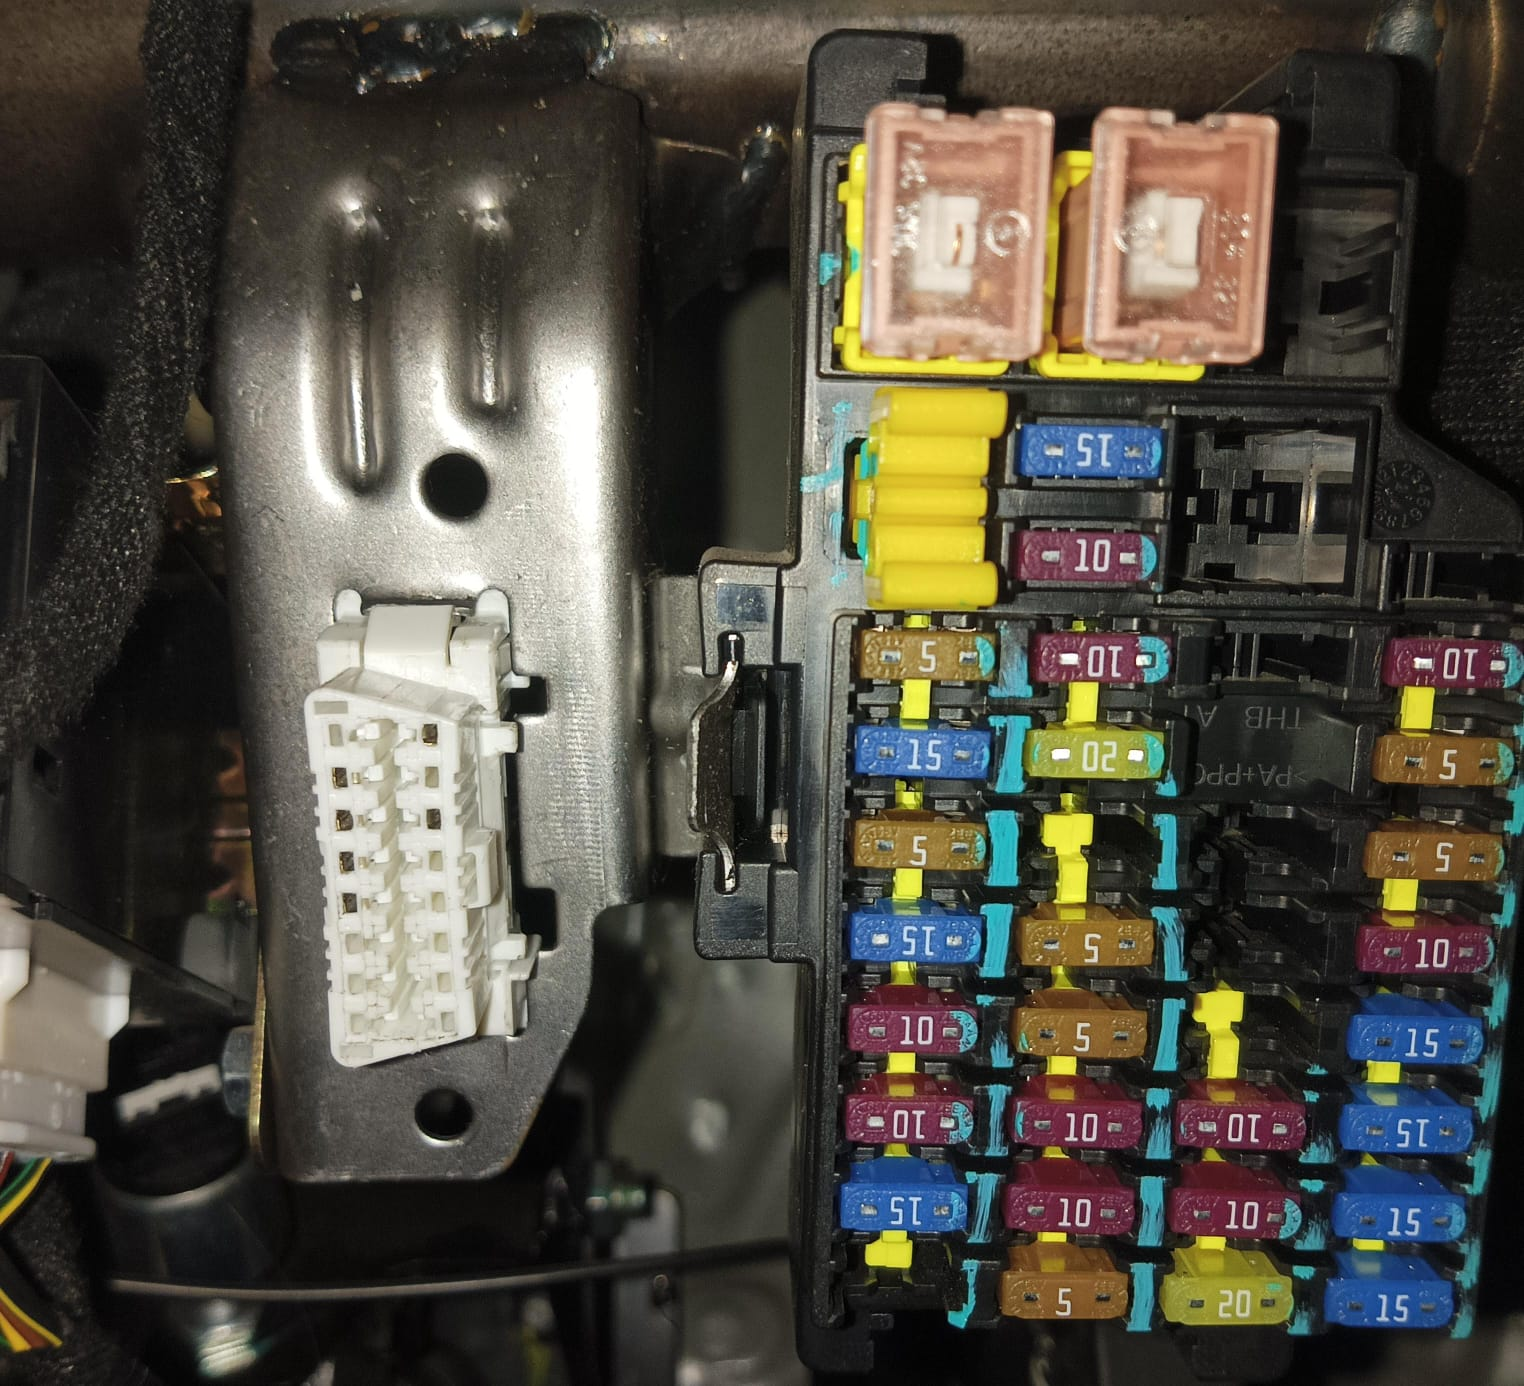
\includegraphics[width=0.55\textwidth]{Images/OBD_CON.jpeg}
		};
		
		% ------------------------------------------------
		% Conector OBD2 (Hembra) - Izquierda
		% ------------------------------------------------
		\node[
		draw=blue,
		very thick,
		rounded corners=3pt,
		fill=white,
		align=center,
		font=\bfseries,
		minimum width=3.8cm,
		minimum height=0.8cm
		] (obd) at ([xshift=-1.0cm,yshift=-2.0cm]foto.north west)
		{Conector OBD2\\(Hembra)};
		
		\draw[
		->,
		blue,
		very thick
		]
		(obd.east)
		-- ([xshift=2.0cm,yshift=-3.8cm]foto.north west);
		
		% ------------------------------------------------
		% 2do Tablero de Fusibles - Derecha
		% ------------------------------------------------
		\node[
		draw=red,
		very thick,
		rounded corners=3pt,
		fill=white,
		align=center,
		font=\bfseries,
		minimum width=3.8cm,
		minimum height=0.8cm
		] (fusibles) at ([xshift=1.0cm,yshift=-2.0cm]foto.north east)
		{2do Tablero de\\Fusibles};
		
		\draw[
		->,
		red,
		very thick
		]
		(fusibles.west)
		-- ([xshift=-2.8cm,yshift=-3.0cm]foto.north east);
		
	\end{tikzpicture}
	
	\vspace{2pt}
	{\footnotesize\textit{Nota.} Vista general del dispositivo dentro del habitáculo del vehículo. Elaboración propia.}
\end{figure}

Con el objetivo de que el dispositivo se instale de manera que no obstruye los controles del conductor y permite el acceso visual a la pantalla OLED durante la conducción.

\section{Configuración del entorno de pruebas}

\subsection{Vehículos utilizados para la validación}

La validación experimental se realiza sobre dos vehículos con arquitecturas de motor distintas. Esto permite evaluar la capacidad de generalización del método Speed-Density ante diferentes configuraciones de inyección y gestión electrónica. La Tabla~\ref{tab:vehiculos} resume sus características principales.

\begin{table}[H]
	\centering
	\captionsetup{labelformat=simple, labelsep=newline, textfont=it, labelfont=bf, justification=raggedright, singlelinecheck=false}
	\caption{Vehículos utilizados en la fase de validación experimental}
	\label{tab:vehiculos}
	\begin{tabularx}{\textwidth}{>{\raggedright\arraybackslash}p{4cm} X X}
		\toprule
		\rowcolor[rgb]{0.851, 0.851, 0.851}
		Característica & Changan Honor & Nissan Vanette \\
		\midrule
		Año de fabricación & 2023 & 2018 \\
		Cilindrada & 1298 mL & 1626 mL \\
		Capacidad de tanque & 40 L & 60 L \\
		Tipo de inyección & Electrónica & Electrónica \\
		Combustible & Gasolina & Gasolina \\
		Protocolo OBD-II & ISO 15765-4 & ISO 15765-4 \\
		Kilometraje aproximado & 5210 & 98765 \\
		Uso habitual & Particular y/o comercial & Cargamento \\
		\bottomrule
	\end{tabularx}
	\vspace{2mm}
	\\
	\begin{minipage}{\linewidth}
		\small
		\textit{Nota.} Ficha técnica comparativa de las unidades vehiculares empleadas para las pruebas de lectura de datos en el bus CAN y la recolección en campo.
	\end{minipage}
\end{table}

La diferencia de antigüedad entre ambos vehículos (2023 frente a 2018) permite además evaluar el comportamiento del sistema frente a posibles variaciones en la calibración de fábrica de los sensores MAP y en el desgaste mecánico propio de un motor con mayor kilometraje.

\begin{figure}[H]
	\centering
	\caption{Vehículos de prueba utilizados en la validación experimental}
	\label{fig:vehiculos_prueba}
	\begin{subfigure}[t]{0.48\textwidth}
		\centering
		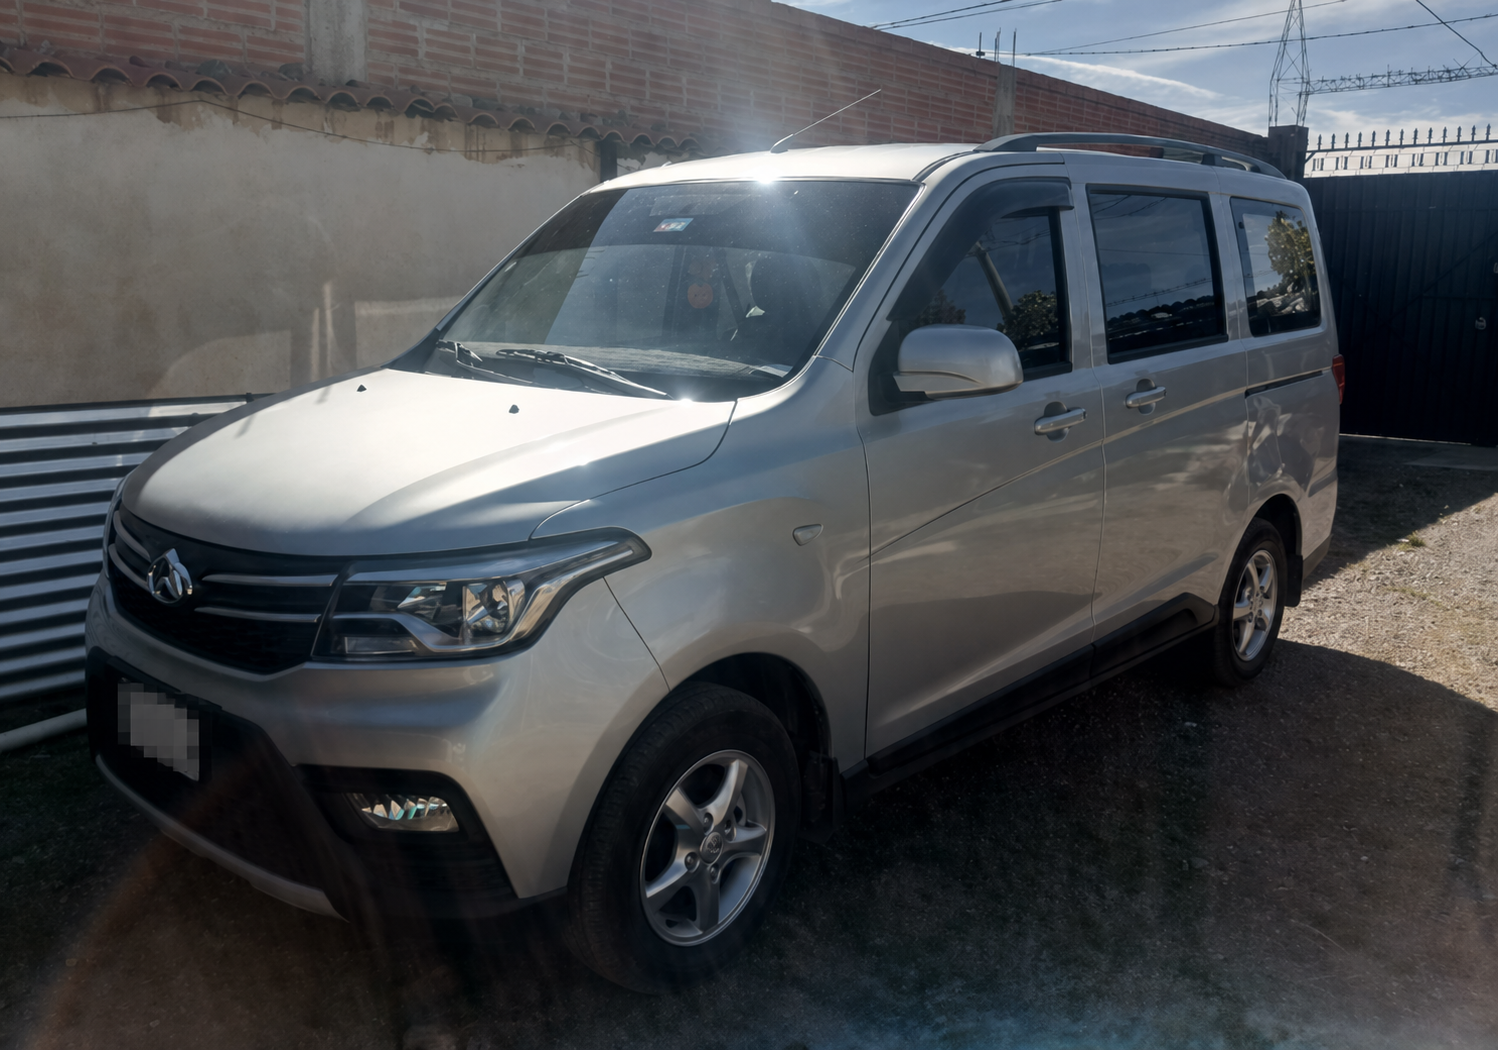
\includegraphics[width=\textwidth]{Images/changan.png}
		\caption{Changan Honor (2023)}
		\label{fig:foto_changan}
	\end{subfigure}
	\hfill
	\begin{subfigure}[t]{0.48\textwidth}
		\centering
		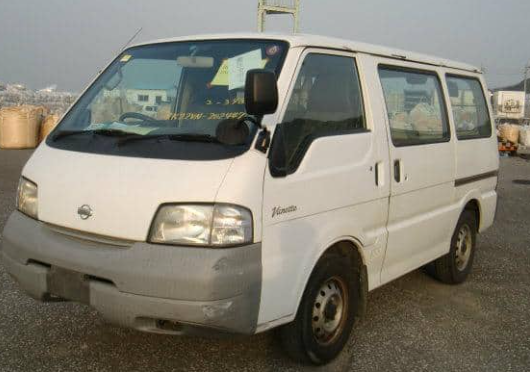
\includegraphics[width=\textwidth]{Images/vanette.png}
		\caption{Nissan Vanette (2018)}
		\label{fig:foto_vanette}
	\end{subfigure}
	\vspace{2pt}
	\\
	{\footnotesize\textit{Nota.} Placa del Changan Honor cubierta por privacidad. Elaboración propia.}
\end{figure}

\subsection{Configuración del adaptador ELM327 como referencia de validación}
\label{sec:elm327_ref}

El adaptador comercial ELM327 (Figura~\ref{fig:elm327_bluetooth}) se emplea como dispositivo de referencia para validar el correcto funcionamiento y la adquisición de datos del sistema desarrollado. Debido a su amplia difusión en la decodificación de protocolos OBD-II, este adaptador permite contrastar las lecturas de los parámetros del motor en tiempo real obtenidos por el prototipo propuesto. Para las pruebas de campo, el ELM327 se configura en modo de comunicación Bluetooth, forzando la selección del protocolo ISO 15765-4 (CAN a 500\,kbps, ID de 11 bits) de manera manual para optimizar los tiempos de inicialización y evitar el proceso de autodetección en cada conexión.

Como herramienta comercial de evaluación se utiliza la aplicación \textit{Car Scanner ELM OBD2}, la cual procesa la información enviada por el ELM327 para calcular el consumo instantáneo y acumulado a partir de las mismas variables del bus CAN (como las RPM, la presión absoluta del colector de admisión MAP y la velocidad del vehículo).

Conviene precisar que tanto el sistema propuesto como la solución basada en el ELM327 calculan el consumo de combustible mediante estimaciones indirectas (método \textit{Speed-Density}) basadas en las señales recopiladas por el bus CAN, y no mediante una medición de flujo directo de gasolina. Así, el cotejo entre ambos equipos representa una prueba de concordancia entre dos plataformas de decodificación.

\textit{Limitación de conexión simultánea.} En las pruebas de campo se verificó que el sistema propio y el adaptador ELM327 no pueden mantener ambos una comunicación estable con la ECU del vehículo al conectarse al mismo tiempo al puerto OBD-II: únicamente uno de los dos dispositivos logra establecer y sostener la sesión de diagnóstico. En consecuencia, la comparación entre ambos no se realiza sobre una única sesión simultánea, sino recorriendo el mismo trayecto dos veces de forma consecutiva (primero con el sistema propio conectado en solitario y, luego, inmediatamente después, con el ELM327 en solitario), manteniendo en lo posible las mismas condiciones de tráfico, ruta y estilo de conducción entre ambas pasadas. Esto introduce una fuente adicional de variabilidad entre las dos lecturas que no proviene de los instrumentos en sí, sino de la imposibilidad de repetir exactamente el mismo tránsito dos veces; se documenta aquí como una limitación metodológica explícita del estudio. Para obtener una referencia de consumo que no dependa de esta limitación ni de ningún método de estimación electrónica, las lecturas de ambos dispositivos se complementan con mediciones volumétricas directas mediante el método de tanque lleno a tanque lleno (Sección~\ref{sec:protocolo_tanque}), realizadas con el sistema propio conectado de forma continua durante todo el trayecto real, tal como se detalla en la Sección~\ref{sec:validacion_cuantitativa}.

% --- FIGURA DE REFERENCIA DEL ELM327 ---
\begin{figure}[htbp]
	\centering
	\caption{Adaptador comercial ELM327 Bluetooth utilizado para la validación de lecturas OBD-II.}
	\label{fig:elm327_bluetooth}
	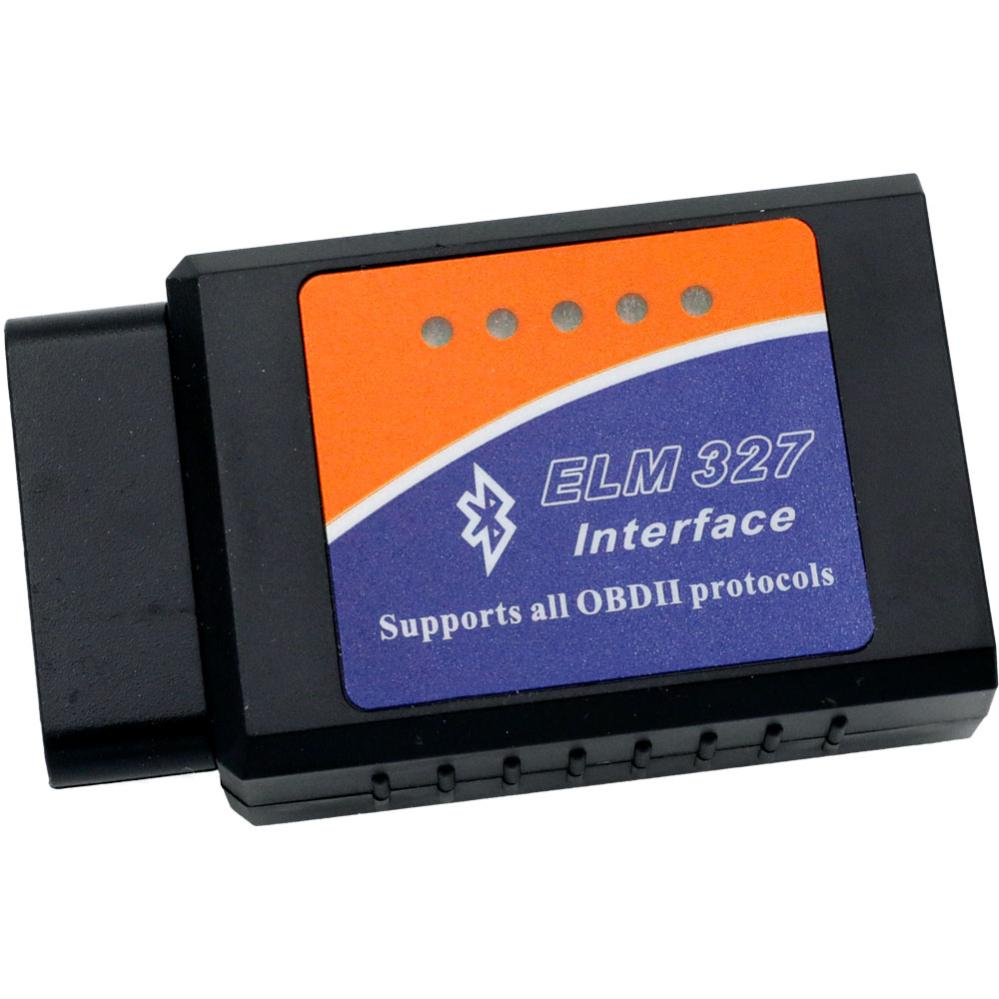
\includegraphics[width=0.45\textwidth]{Images/elm327.jpg} % Ajusta la ruta y nombre de tu imagen
	\\
	\vspace{2pt}
	{\footnotesize\textit{Nota.} Scanner comercial ELM327.}
\end{figure}

\subsection{Puesta en marcha del firmware y verificación inicial}

Antes de cada sesión de pruebas, se ejecuta una rutina de verificación inicial que confirma la correcta inicialización del controlador TWAI (sin errores de bus-off), el montaje del sistema de archivos en la tarjeta MicroSD, la sincronización horaria del registro de datos y la visualización de al menos un parámetro en tiempo real (RPM o velocidad) en la pantalla OLED. La confirmación del correcto funcionamiento de cada uno de estos subsistemas se realiza mediante indicadores LED integrados en el módulo (Tabla~\ref{tab:checklist_arranque}); así se descarta en segundos una falla de montaje antes de invertir tiempo de trayecto en una sesión de prueba inválida.

\begin{table}[H]
	\centering
	\captionsetup{labelformat=simple, labelsep=newline, textfont=it, labelfont=bf, justification=raggedright, singlelinecheck=false}
	\caption{Lista de verificación previa a cada sesión de pruebas}
	\label{tab:checklist_arranque}
	\begin{tabularx}{\textwidth}{>{\raggedright\arraybackslash}p{4.2cm} X >{\centering\arraybackslash}p{2.6cm}}
		\toprule
		\rowcolor[rgb]{0.851, 0.851, 0.851}
		Verificación & Indicador esperado & Resultado \\
		\midrule
		Bus CAN inicializado, sin bus-off & LED CAN encendido fijo tras conectar el contacto & \checkmark \\
		Tarjeta MicroSD montada & LED SD parpadea al escribir (una vez por segundo) &\checkmark \\
		Servidor web activo & LED Server encendido; SSID \texttt{ESP32\_OBD2} visible al buscar redes &\checkmark \\
		Ningún error activo & LED Error apagado (sin patrón de parpadeo) & \checkmark \\
		Parámetro en vivo visible & RPM o velocidad actualizándose en el OLED & \checkmark \\
		\bottomrule
	\end{tabularx}
	\vspace{2mm}
	\\
	\begin{minipage}{\linewidth}
		\small
		\textit{Nota.} Se completa con \checkmark~(correcto) o \texttt{X} (falla, con la causa anotada aparte) al inicio de cada sesión, antes de arrancar el vehículo. Si el LED de error está encendido, el código de parpadeo (Sección~4.3 del Capítulo~3, \texttt{status\_leds.cpp}) indica el subsistema que falló.
	\end{minipage}
\end{table}

\subsection{Herramientas y procesamiento de datos para el análisis}
\label{sec:herramientas_analisis}

Cada sesión de prueba produce datos de tres fuentes distintas, que deben combinarse fuera del dispositivo para calcular las métricas de la Sección~\ref{sec:validacion_cuantitativa}:

\begin{enumerate}
	\item \textbf{CSV del sistema propio}, descargado desde el panel web (\texttt{/api/download}) al finalizar cada trayecto, o directamente de la tarjeta MicroSD. Contiene una fila por segundo con las columnas descritas en el Capítulo~3 (\texttt{trip\_km}, \texttt{trip\_fuel\_L}, \texttt{instant\_L100km}, \texttt{baro\_kpa}, entre otras).
	\item \textbf{Registro del ELM327 + \textit{Car Scanner}}, exportado como CSV o KML/GPX desde la propia aplicación (opción de exportación en el historial de sesión), con marcas de tiempo y consumo instantáneo/acumulado calculado por la app.
	\item \textbf{Bitácora manual de aforo}, un cuaderno o planilla con hora, odómetro y litros cargados en cada llenado de tanque (Sección~\ref{sec:protocolo_tanque}).
\end{enumerate}

El análisis se centraliza en un script de Python (\texttt{pandas} para leer y alinear los CSV por marca de tiempo, \texttt{numpy}/\texttt{scipy.stats} para las métricas estadísticas) en vez de calcularse a mano: de esta forma el proceso es reproducible, permite reprocesar todos los trayectos si se detecta un error, y deja un registro auditable de exactamente cómo se obtuvo cada número de la Tabla~\ref{tab:metricas_validacion}. Este y el resto de los scripts de análisis usados en el capítulo se encuentran en la carpeta \texttt{CODIGOS/} del repositorio de GitHub del proyecto \citep{CalleGitHub2026}, junto con el firmware del dispositivo. Las funciones utilizadas para cada métrica son las siguientes:

\begin{itemize}
	\item RMSE y MAE: \texttt{numpy.sqrt(numpy.mean((est-ref)**2))} y \texttt{numpy.mean(numpy.abs(est-ref))} respectivamente, sobre los pares (estimado, referencia) de cada trayecto o punto de muestreo.
	\item MAPE: \texttt{numpy.mean(numpy.abs((est-ref)/ref))*100}, evitando dividir entre valores de referencia cercanos a cero (por ejemplo, excluyendo muestras con el vehículo detenido).
	\item Pearson $r$ y $R^2$: \texttt{scipy.stats.pearsonr(est, ref)}; $R^2$ es el cuadrado del coeficiente devuelto, o directamente el de una regresión lineal con \texttt{scipy.stats.linregress}.
	\item Bland-Altman: calcular por muestra la diferencia $d = est - ref$ y el promedio $m = (est+ref)/2$; el sesgo medio es $\bar d$ y los límites de concordancia son $\bar d \pm 1{,}96\,s_d$, con $s_d$ la desviación estándar de $d$. Un gráfico de dispersión de $d$ contra $m$, con esas tres líneas horizontales, es la figura estándar de este análisis.
	\item Repetibilidad: coeficiente de variación $CV = s/\bar{x}$ del sistema propio sobre las repeticiones del mismo trayecto (Sección~\ref{sec:protocolo_tanque}), expresado en porcentaje.
\end{itemize}

\section{Pruebas experimentales}

Esta sección describe la metodología seguida para cada tipo de prueba. En todos los casos se recomienda repetir cada prueba al menos 3 veces para poder estimar la variabilidad de la medición y no depender de una sola observación.

\subsection{Validación de la comunicación CAN (ESP32 vs. ELM327)}

Esta prueba verifica que el sistema propuesto decodifica correctamente las tramas de la ECU, con una tasa de éxito comparable a la del adaptador comercial. Dado que, como se explicó en la Sección~\ref{sec:elm327_ref}, ambos dispositivos no pueden mantener una sesión OBD-II estable conectados simultáneamente al mismo puerto, esta verificación se realiza en dos sesiones separadas y consecutivas —motor encendido en ralentí, ventana de tiempo fija (por ejemplo, 5 minutos) para cada dispositivo—, registrando el número de tramas recibidas, la tasa de tramas perdidas o corruptas, y la latencia entre solicitud y respuesta de cada uno por separado. La Tabla~\ref{tab:validacion_can} propone el formato de registro; la columna ``Diferencia'' compara el desempeño de cada dispositivo en su propia sesión, no una medición conjunta.

\begin{table}[H]
	\centering
	\captionsetup{labelformat=simple, labelsep=newline, textfont=it, labelfont=bf, justification=raggedright, singlelinecheck=false}
	\caption{Formato de registro para la validación de la comunicación CAN (sesiones separadas)}
	\label{tab:validacion_can}
	\begin{tabularx}{\textwidth}{X >{\centering\arraybackslash}p{3.5cm} >{\centering\arraybackslash}p{2.5cm} >{\centering\arraybackslash}p{2.5cm}}
		\toprule
		\rowcolor[rgb]{0.851, 0.851, 0.851}
		Parámetro & ESP32-S3 (sesión propia) & ELM327 (sesión separada) & Diferencia \\
		\midrule
		Tramas recibidas en 5 min & 2936 & 1712 & 1224 \\
		Tramas con error de CRC & 0 & 34 & 34 \\
		Latencia promedio (ms) & 2.2 & 231.4 & 229.2 \\
		\bottomrule
	\end{tabularx}
	\vspace{2mm}
	\\
	\begin{minipage}{\linewidth}
		\small
		\textit{Nota.} Cada columna de dispositivo corresponde a una sesión de conexión independiente (Sección~\ref{sec:elm327_ref}), con el vehículo en ralentí para minimizar la variabilidad entre ambas ventanas de medición.
	\end{minipage}
\end{table}

\subsubsection*{Herramientas de medición}

Los valores de la Tabla~\ref{tab:validacion_can} se obtuvieron con dos programas de referencia construidos específicamente para esta prueba, uno por dispositivo, ya que ninguno de los dos expone estas métricas de forma nativa:

\begin{itemize}
	\item \textbf{ESP32-S3} (\texttt{CODIGOS/can\_bench\_tool/}): un proyecto PlatformIO independiente del firmware de producción que, durante 5~minutos, solicita repetidamente el PID~0x0C (RPM), el único PID obligatorio en todo ECU OBD-II (así se aísla el desempeño de la comunicación en sí de la disponibilidad de un PID particular), y mide el tiempo entre cada solicitud y su respuesta directamente sobre el controlador TWAI nativo.
	\item \textbf{ELM327} (\texttt{CODIGOS/elm327\_bench.py}): un script en Python que se conecta al adaptador por Bluetooth y le envía el mismo PID mediante comandos AT estándar, sin pasar por la aplicación comercial, para medir la misma ventana de 5~minutos bajo las mismas condiciones de solicitud.
\end{itemize}

\begin{figure}[H]
	\centering
	\caption{Núcleo de medición de latencia en el benchmark del ESP32-S3, \texttt{can\_bench\_tool/src/main.cpp}.}
	\label{fig:bench_esp32}
	\begin{lstlisting}[language=C++, basicstyle=\fontsize{9}{10}\ttfamily, breaklines=true]
uint32_t reqStartUs = micros();
requestsSent++;

if (sendPidRequest(PID_TO_TEST) && waitForResponse(PID_TO_TEST, RESPONSE_TIMEOUT_MS)) {
  responsesOk++;
  latencySumUs += (uint64_t)(micros() - reqStartUs);
}

uint32_t alerts = 0;
if (twai_read_alerts(&alerts, 0) == ESP_OK && alerts != 0) {
  if (alerts & (TWAI_ALERT_BUS_ERROR | TWAI_ALERT_ERR_PASS | TWAI_ALERT_BUS_OFF)) {
    errorFrames++;
  }
}
	\end{lstlisting}
	\begin{minipage}{\linewidth}
		\small
		\textit{Nota.} La latencia se mide con \texttt{micros()} entre el envío de la solicitud y la recepción de la trama de respuesta válida; los errores se cuentan a partir de las alertas del propio controlador TWAI (\texttt{ESP-IDF}), no de una re-implementación manual de detección de errores de bus.
	\end{minipage}
\end{figure}

\begin{figure}[H]
	\centering
	\caption{Núcleo de medición y clasificación de respuestas en el benchmark del ELM327, \texttt{elm327\_bench.py}.}
	\label{fig:bench_elm327}
	\begin{lstlisting}[language=Python, basicstyle=\fontsize{9}{10}\ttfamily, breaklines=true]
t0 = time.time()
ser.reset_input_buffer()
ser.write(b"010C\r")
requests_sent += 1

resp = ser.read(64).decode(errors="ignore")
elapsed = time.time() - t0
resp_clean = resp.replace("\r", " ").upper()

if "NO DATA" in resp_clean or "ERROR" in resp_clean or "BUS" in resp_clean:
    error_frames += 1
elif "41 0C" in resp_clean:
    responses_ok += 1
    latencies.append(elapsed)
	\end{lstlisting}
	\begin{minipage}{\linewidth}
		\small
		\textit{Nota.} La latencia incluye, a diferencia de la medición del ESP32-S3, el tiempo de procesamiento interno del ELM327 (traducción de comandos AT a tramas CAN) y de la pila Bluetooth del sistema operativo, no solo el tiempo de bus.
	\end{minipage}
\end{figure}

\subsection{Verificación de comunicación OBD-II mediante PIDs}

La verificación de la comunicación con cada vehículo 
se realizó mediante la solicitud y recepción de 
parámetros estándar definidos por el protocolo 
OBD-II (SAE J1979), conocidos como \textit{Parameter 
	IDs} (PIDs), utilizando el modo de servicio 
\texttt{0x01} (datos en tiempo real).

El procedimiento consistió en enviar tramas CAN 
con el formato estándar OBD-II (\texttt{0x7DF} 
como ID de solicitud broadcast) y capturar la 
respuesta de la ECU de cada vehículo 
(\texttt{0x7E8}). Los PIDs reportados como disponibles por cada 
vehículo fueron contrastados contra la tabla 
de referencia del modo 01 (Apéndice A) 
y el análisis matemático de resolución por PID 
disponible, obteniendo los 
resultados de disponibilidad resumidos en la 
Tabla~\ref{tab:pids_verificacion}, un detalle mas completo se presenta en el Apéndice O.

\begin{table}[H]
	\centering
	\caption{PIDs consultados y disponibilidad por vehículo.}
	\label{tab:pids_verificacion}
	\begin{tabular}{clccc}
		\toprule
		\rowcolor[rgb]{.851,.851,.851}
		\textbf{PID} & \textbf{Parámetro} & \textbf{Unidad} & \textbf{Changan Honor} & \textbf{Nissan Vanette} \\
		\midrule
		\texttt{0x0C} & Régimen del motor (RPM) & rpm & \checkmark & \checkmark \\
		\texttt{0x0D} & Velocidad del vehículo & km/h & \checkmark & \checkmark \\
		\texttt{0x10} & Flujo másico de aire (MAF) & g/s &  & \checkmark \\
		\texttt{0x05} & Temperatura del refrigerante & °C & \checkmark & \checkmark \\
		\texttt{0x11} & Posición del acelerador & \% & \checkmark & \checkmark \\
		\bottomrule
	\end{tabular}
	\vskip 0.15cm
	{\footnotesize \textit{Nota.} PIDs verificados mediante el escaneo de la Figura~\ref{fig:codigo_scanner_obd2}.}
\end{table}

La disponibilidad del PID \texttt{0x10} (MAF) 
en ambos vehículos es crítica para el sistema,
ya que es el parámetro base para el
cálculo del consumo de combustible, conforme
a la fórmula de decodificación definida por 
el estándar SAE J1979 \citep{saej1979}.

\subsection{Pruebas del modelo Speed-Density}

Se realizan pruebas estáticas a régimen de motor controlado (en ralentí y en pasos de 1500, 2500 y 3500\,rpm, sin carga en las ruedas) con el fin de aislar el comportamiento del modelo Speed-Density de las variables dinámicas de conducción. El primer punto no se fija a un número redondo arbitrario (por ejemplo, 800\,rpm): el regulador de ralentí de cada motor tiene su propio piso, por debajo del cual el motor no puede sostenerse sin calarse —en el Nissan Vanette utilizado, ese piso se ubicó experimentalmente entre 960 y 980\,rpm—, así que el primer punto se toma directamente como el ralentí real medido al inicio de la prueba. En cada punto se registra el caudal de aire estimado por el sistema propio y se contrasta contra el valor de referencia reportado por la ECU a través del PID estándar de MAF, cuando el vehículo lo soporta.

Esta comparación directa punto a punto solo es posible en el \textbf{Nissan Vanette}, que sí reporta el PID 0x10 (Tabla~\ref{tab:pids_verificacion}). El \textbf{Changan Honor} no dispone de sensor MAF (es, de hecho, la razón por la que este proyecto necesita el método Speed-Density en primer lugar, Sección~\ref{subsec:soporte_pids} del Capítulo~3), de modo que no existe una referencia directa de caudal de aire para ese vehículo en esta prueba estática. Su exactitud se evalúa entonces de forma indirecta, aguas abajo, a través de la comparación de consumo acumulado contra el aforo real por tanque lleno (Sección~\ref{sec:protocolo_tanque}), que sí aplica a ambos vehículos por igual.

\subsubsection*{Herramienta de medición}

A diferencia de la validación de comunicación CAN de la sección anterior, esta prueba no compara un dispositivo contra otro, sino una \emph{estimación} contra una \emph{referencia}, y ambas se calculan a partir de las mismas lecturas de RPM, MAP e IAT tomadas en el mismo instante. Por eso aquí basta con el \textbf{ELM327 solo}, hablado directamente por un script en Python (\texttt{CODIGOS/speed\_density\_bench.py} en el repositorio del proyecto \citep{CalleGitHub2026}): en cada ciclo solicita RPM (PID~0x0C), MAP (PID~0x0B), IAT (PID~0x0F) y MAF real (PID~0x10), y con las tres primeras calcula el MAF estimado usando exactamente la misma fórmula y tabla de eficiencia volumétrica (VE) que el firmware de producción (\texttt{fuel\_calc.cpp}). Al no requerir una segunda sesión OBD-II en paralelo, esta prueba queda al margen de la limitación de conexión simultánea documentada en la Sección~\ref{sec:elm327_ref}.

\begin{figure}[H]
	\centering
	\caption{Cálculo del MAF estimado en \texttt{speed\_density\_bench.py}, réplica en Python de la fórmula de \texttt{fuel\_calc.cpp}.}
	\label{fig:bench_speed_density}
	\begin{lstlisting}[language=Python, basicstyle=\fontsize{9}{10}\ttfamily, breaklines=true]
def maf_estimado_gs(rpm, map_kpa, iat_c):
    ve = ve_for_rpm(rpm)          # misma tabla VE que kVeTable en fuel_calc.cpp
    iat_k = iat_c + 273.15
    if iat_k < 233.15 or iat_k > 373.15:
        iat_k = 288.15             # misma guarda que el firmware
    maf = (ve / 100.0) * rpm * map_kpa * ENGINE_DISPLACEMENT_L * MM_AIR \
          / (2.0 * R * iat_k * 60.0)
    return max(maf, 0.0)
	\end{lstlisting}
	\begin{minipage}{\linewidth}
		\small
		\textit{Nota.} \texttt{ENGINE\_DISPLACEMENT\_L}, la tabla \texttt{VE\_TABLE} y las constantes \texttt{MM\_AIR}/\texttt{R} son una copia literal de los valores de \texttt{config.h} y \texttt{fuel\_calc.cpp}, de modo que la estimación calculada en la prueba es la misma que produciría el equipo embarcado ante las mismas lecturas.
	\end{minipage}
\end{figure}

Al iniciar, el script mide el ralentí real promediando varias lecturas de RPM antes de comenzar a clasificar muestras, y lo antepone a los otros tres puntos fijos (1500, 2500 y 3500~rpm) como el primer objetivo de la prueba. Cada muestra se clasifica según el punto de régimen objetivo más cercano, con tolerancia de $\pm$100~rpm, y se descarta si no cae dentro de esa tolerancia; al finalizar la prueba el script promedia el MAF estimado y el MAF de referencia dentro de cada punto y calcula el error porcentual entre ambos.

\begin{table}[H]
	\centering
	\caption{Comparación del MAF estimado por el modelo Speed-Density frente al MAF de referencia de la ECU (PID 0x10), Nissan Vanette}
	\label{tab:speed_density_resultados}
	\begin{tabular}{ccccc}
		\toprule
		\rowcolor[rgb]{0.851, 0.851, 0.851}
		\textbf{RPM} & \textbf{n muestras} & \textbf{MAF estimado (g/s)} & \textbf{MAF ref. (g/s)} & \textbf{Error (\%)} \\
		\midrule
		Ralentí (940\,rpm) & 22 & 2,04 & 2,68 & $-23{,}7$ \\
		1500 & 25 & 3,52 & 3,90 & $-9{,}8$ \\
		2500 & 22 & 7,21 & 6,89 & $+4{,}7$ \\
		3500 & 20 & 11,74 & 9,90 & $+18{,}7$ \\
		\bottomrule
	\end{tabular}
	\vskip 0.15cm
	{\footnotesize \textit{Nota.} Valores promedio por punto de régimen, obtenidos con \texttt{speed\_density\_bench.py} y registrados en \texttt{speed\_density\_log.csv}. Error (\%) = (MAF estimado $-$ MAF referencia) / MAF referencia $\times$ 100.}
\end{table}

\begin{figure}[H]
	\centering
	\caption{Comparación del caudal de aire estimado por el modelo Speed-Density frente al valor de referencia de la ECU, por régimen de motor}
	\label{fig:speed_density_scatter}
	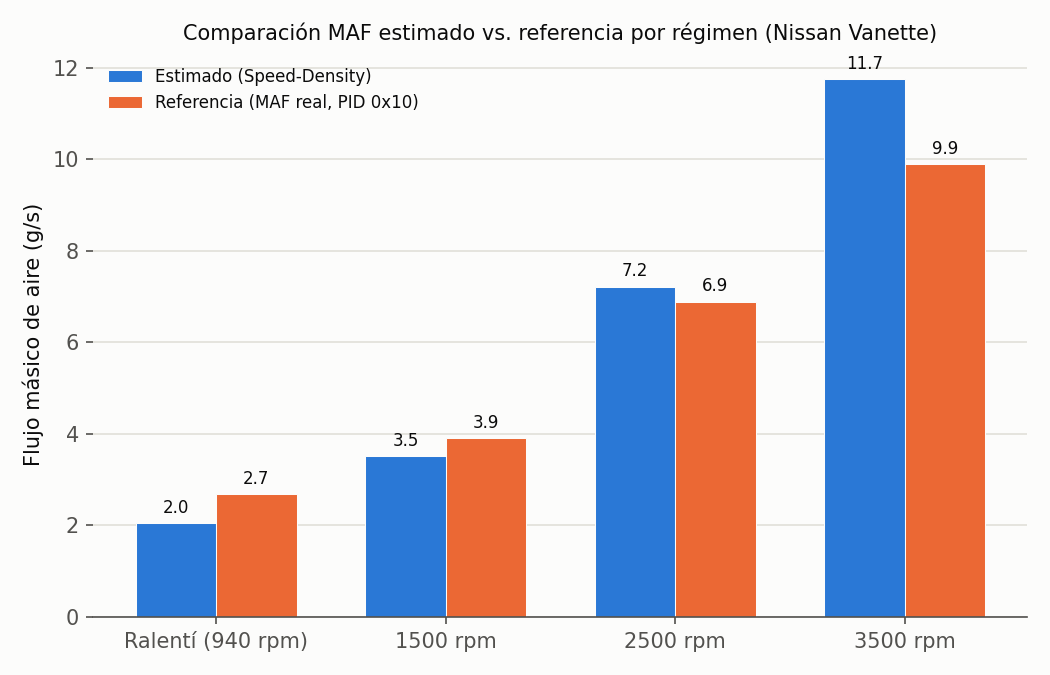
\includegraphics[width=0.8\textwidth]{Images/figura_4_9_speed_density.png}

	\vspace{2pt}
	{\footnotesize\textit{Nota.} Gráfico de barras agrupadas, un par de barras (estimado / referencia) por cada uno de los cuatro regímenes evaluados. Se prefiere sobre un diagrama de dispersión porque el diseño experimental produce cuatro promedios discretos por punto de régimen, no una nube de muestras continuas cuya correlación interese visualizar: precisamente el caso de uso de las barras agrupadas frente a la dispersión. Elaboración propia.}
\end{figure}

\subsubsection*{Calibración del modelo Speed-Density}
\label{sec:calibracion_speed_density}

Los resultados de la Tabla~\ref{tab:speed_density_resultados} muestran un error grande y, más importante, de \emph{signo variable} entre regímenes: el modelo subestima el caudal de aire en ralentí y a 1500\,rpm ($-23{,}7\,\%$ y $-9{,}8\,\%$), pero lo sobrestima a 2500 y 3500\,rpm ($+4{,}7\,\%$ y $+18{,}7\,\%$). Un sesgo de signo constante podría explicarse por un solo factor de escala mal calibrado (por ejemplo, la cilindrada); un sesgo que cambia de signo con el régimen, en cambio, apunta a que la \emph{forma} de la curva de eficiencia volumétrica (VE) usada por el modelo no corresponde a la de este motor en particular. Al notar un error de esta magnitud, se procede a calibrar el sistema con los mismos datos de la Tabla~\ref{tab:speed_density_resultados}, en vez de aceptar la tabla VE genérica con la que partió el diseño.

La revisión encontró además un segundo problema, independiente del anterior: la constante \texttt{ENGINE\_DISPLACEMENT\_L} del firmware (\texttt{config.h}) estaba fijada en 1,6\,L, mientras que la cilindrada real del Nissan Vanette, según su ficha técnica (Tabla~\ref{tab:vehiculos}), es de 1626\,mL. Ambas correcciones —cilindrada real y tabla VE calibrada— se aplican juntas antes de recalcular.

\paragraph{Método de calibración.} La ecuación de \texttt{fuel\_calc.cpp} (Sección~\ref{sec:speeddensity} del Capítulo~3) se invierte algebraicamente para despejar la VE que, dada una muestra real de RPM, MAP e IAT, hace que el MAF estimado coincida exactamente con el MAF de referencia:

\begin{equation}
	VE_{\text{requerida}} = \frac{MAF_{\text{ref}} \cdot 100 \cdot 2 \cdot R \cdot T_{IAT} \cdot 60}{RPM \cdot P_{MAP} \cdot V_d \cdot 28{,}97}
	\label{eq:ve_calibracion}
\end{equation}

Esta inversión se aplica muestra por muestra sobre \texttt{speed\_density\_log.csv} y se promedia por punto de régimen mediante \texttt{CODIGOS/calibrate\_ve\_table.py}, un script nuevo e independiente de \texttt{speed\_density\_bench.py} (no requiere el vehículo ni el ELM327, solo el CSV ya grabado). La Tabla~\ref{tab:ve_calibracion} resume la VE que exigía la tabla genérica original frente a la VE real requerida en cada punto.

\begin{table}[H]
	\centering
	\caption{Eficiencia volumétrica (VE) genérica frente a la VE real requerida, por punto de régimen}
	\label{tab:ve_calibracion}
	\begin{tabular}{cccc}
		\toprule
		\rowcolor[rgb]{0.851, 0.851, 0.851}
		\textbf{Punto} & \textbf{RPM promedio real} & \textbf{VE genérica (\%)} & \textbf{VE requerida (\%)} \\
		\midrule
		Ralentí & 936,3 & 64,1 & 82,7 \\
		1500    & 1446,7 & 73,1 & 79,7 \\
		2500    & 2491,6 & 84,9 & 79,7 \\
		3500    & 3483,0 & 87,0 & 72,7 \\
		\bottomrule
	\end{tabular}
	\vskip 0.15cm
	{\footnotesize \textit{Nota.} Calculado con \texttt{calibrate\_ve\_table.py} sobre \texttt{speed\_density\_log.csv}, usando $V_d=1{,}626$\,L. Los puntos 4000/5500/7000\,rpm de \texttt{kVeTable} no se modifican por no contar con datos de prueba en ese rango; quedan documentados como sin calibrar.}
\end{table}

La tabla \texttt{kVeTable} de \texttt{fuel\_calc.cpp} y su copia en \texttt{speed\_density\_bench.py} se actualizan con estos cuatro puntos calibrados, conservando sin cambios los tres puntos superiores (4000/5500/7000\,rpm) por no contarse con mediciones reales en ese rango.

\begin{figure}[H]
	\centering
	\caption{Validación de la tabla VE calibrada frente al MAF de referencia, mismo conjunto de datos de calibración}
	\label{fig:post_calibracion}
	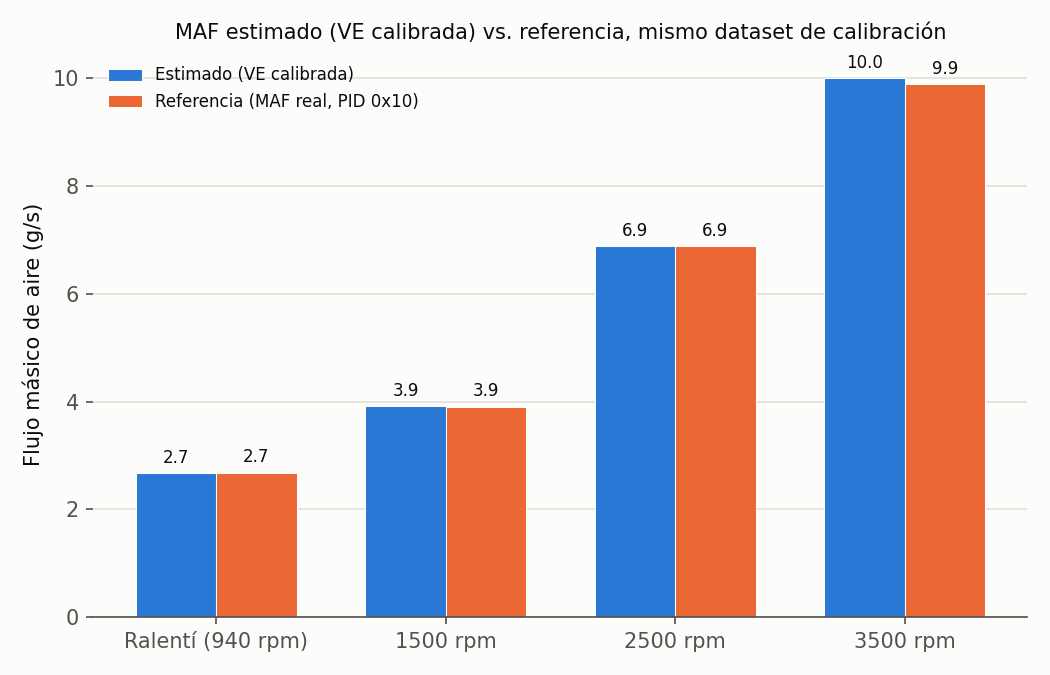
\includegraphics[width=0.8\textwidth]{Images/figura_4_10_post_calibracion.png}

	\vspace{2pt}
	{\footnotesize\textit{Nota.} Generado por \texttt{calibrate\_ve\_table.py} recalculando el MAF estimado de cada muestra con la tabla ya calibrada. El error residual (entre $-0{,}02\,\%$ y $+1{,}03\,\%$ según el punto) confirma que la inversión algebraica se aplicó correctamente, pero \textbf{no} es una validación independiente del modelo: al calibrar y verificar sobre el mismo conjunto de datos, un error cercano a cero es el resultado esperado por construcción, no evidencia de que el modelo generalice a condiciones dinámicas de conducción o a otro rango de régimen. Elaboración propia.}
\end{figure}

Esta limitación metodológica —validar sobre el mismo conjunto de datos con el que se calibró— se resuelve con una segunda prueba, dinámica, descrita a continuación.

\subsubsection*{Prueba dinámica (ruta real)}
\label{sec:sd_prueba_dinamica}

A diferencia de la prueba estática anterior, aquí no se sostiene el motor en puntos fijos de régimen: se conduce una ruta real (arranque, aceleración, crucero a distintas velocidades, frenado) mientras el sistema registra continuamente RPM, MAP, IAT y el MAF real de referencia. El objetivo no es calibrar nada —la tabla VE ya quedó fija en la prueba estática—, sino verificar qué tan bien predice el modelo \emph{ya calibrado} sobre datos que nunca participaron en esa calibración, resolviendo directamente la limitación señalada en la Figura~\ref{fig:post_calibracion}. Al igual que la prueba estática, esta solo aplica al \textbf{Nissan Vanette} (único vehículo con PID 0x10).

\texttt{CODIGOS/speed\_density\_drive\_log.py} realiza este registro: a diferencia de \texttt{speed\_density\_bench.py}, no agrupa las muestras por punto de régimen objetivo ni corta automáticamente (ese criterio, pensado para la prueba estática, cortaría una ruta real apenas el RPM de manejo normal pasara cerca de cualquiera de los 4 puntos fijos), así que aquí simplemente registra cada muestra tal como llega, sin requerir ninguna interacción mientras se maneja. Al finalizar (Ctrl+C), \texttt{CODIGOS/speed\_density\_drive\_validation.py} calcula sobre el registro completo las mismas métricas ya definidas en la Sección~\ref{sec:herramientas_analisis} (RMSE, MAE, MAPE, coeficiente de Pearson) y genera un diagrama de dispersión del MAF estimado frente al de referencia. A diferencia de la Figura~\ref{fig:speed_density_scatter} (barras, 4 promedios discretos), aquí sí corresponde un diagrama de dispersión: el registro de una ruta produce una nube continua de muchas muestras correlacionadas, el caso de uso exacto de ese tipo de gráfico.

\begin{figure}[H]
	\centering
	\caption{Dispersión del MAF estimado frente al MAF de referencia durante una ruta real}
	\label{fig:dispersion_dinamica}
	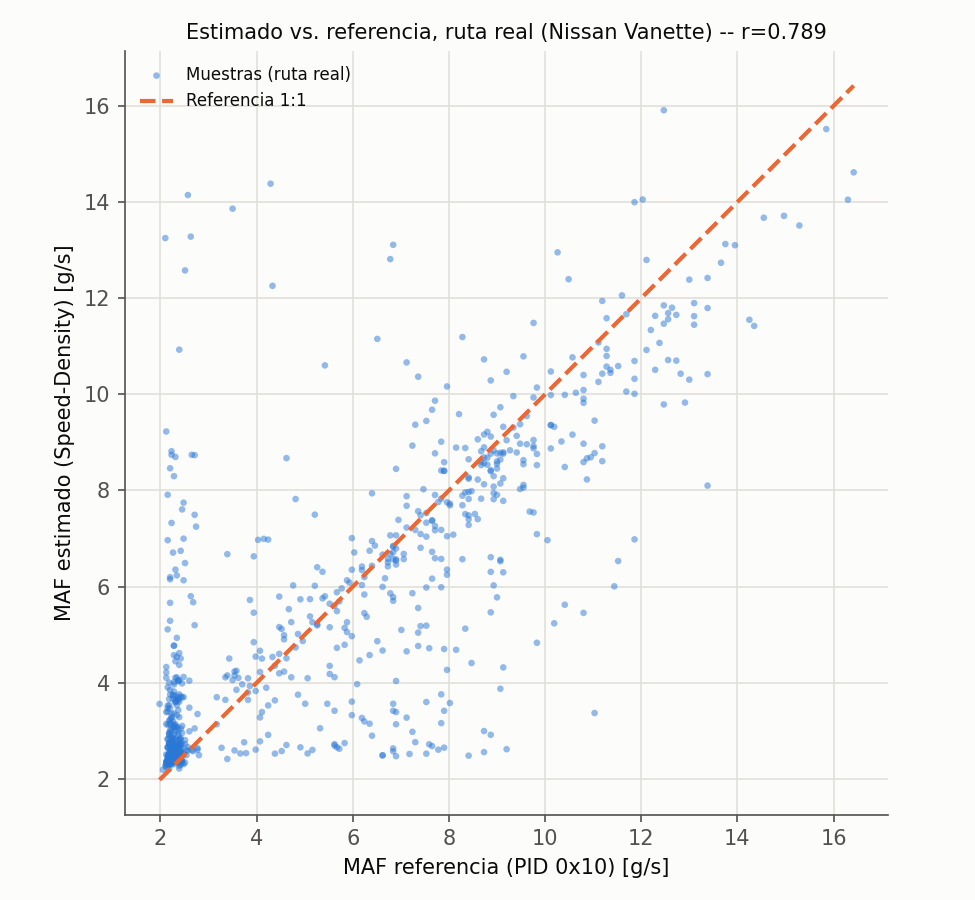
\includegraphics[width=0.7\textwidth]{Images/figura_dispersion_dinamica.png}

	\vspace{2pt}
	{\footnotesize\textit{Nota.} Cada punto es una muestra del registro de ruta; la línea discontinua es la recta 1:1 (predicción perfecta). Elaboración propia.}
\end{figure}

\subsection{Validación del sensor MAP frente a la altitud}
\label{sec:validacion_map_altitud}

A diferencia de una implementación que asumiera una presión de referencia fija
de nivel del mar, el método speed-density de este proyecto usa en cada ciclo
la presión absoluta real del colector (MAP, PID 0x0B) reportada por la propia
ECU, por lo que el cálculo de consumo ya queda corregido por altitud sin
necesitar ningún factor adicional (Sección~\ref{sec:speeddensity} y
Subsección~\ref{subsec:etav-altitud} del Capítulo~3). Lo que sí conviene
verificar en campo es que el \emph{sensor} MAP del vehículo esté bien
calibrado para operar a los $\approx 3\,600$\,msnm de La Paz, ya que un sesgo
de fábrica en ese sensor sí se propagaría al consumo calculado.

La prueba consiste en comparar, con el contacto puesto y el motor apagado
(\textit{key-on, engine-off}, sin vacío de admisión), la lectura de MAP
contra la presión barométrica real. El firmware registra esta última como
\texttt{baro\_kpa} en el CSV y en el panel web (PID 0x33 cuando el vehículo
lo soporta; en su defecto, la estimación del modelo ISA evaluado en
\texttt{SITE\_ALTITUDE\_M}, marcada como tal mediante
\texttt{baro\_is\_estimated}). La Tabla~\ref{tab:validacion_map_altitud}
propone el formato de registro.

\subsubsection*{Herramienta de medición}

Al ser una prueba puntual (motor apagado, sin trayecto de por medio), esta fila de la Tabla~\ref{tab:validacion_map_altitud} se llena con un script independiente, \texttt{CODIGOS/map\_altitude\_report.py}, que se conecta directamente al ELM327 por Bluetooth y no requiere el sistema propio conectado a la vez: solicita el PID~0x0B (MAP) y el PID~0x33 (presión barométrica) un número fijo de veces, promedia ambas lecturas y calcula la diferencia porcentual entre ellas. Si el vehículo no soporta el PID~0x33 —caso que se decide en tiempo de ejecución, no de antemano—, el script recurre al mismo modelo ISA evaluado en \texttt{SITE\_ALTITUDE\_M} que usa el firmware como respaldo (\texttt{isaPressureKpaAt()} en \texttt{can\_obd2.cpp}), replicado con la fórmula idéntica en Python. Cada corrida se ejecuta una vez por vehículo y se anexa a \texttt{map\_altitude\_report.csv}, listo para copiar a la Tabla~\ref{tab:validacion_map_altitud}.

\begin{table}[H]
	\centering
	\captionsetup{labelformat=simple, labelsep=newline, textfont=it, labelfont=bf, justification=raggedright, singlelinecheck=false}
	\caption{Validación del sensor MAP en \textit{key-on, engine-off} frente a la presión barométrica}
	\label{tab:validacion_map_altitud}
	\begin{tabularx}{\textwidth}{X >{\centering\arraybackslash}p{3cm} >{\centering\arraybackslash}p{3cm} >{\centering\arraybackslash}p{3cm}}
		\toprule
		\rowcolor[rgb]{0.851, 0.851, 0.851}
		Vehículo & MAP en KOEO (kPa) & \texttt{baro\_kpa} (kPa) & Diferencia (\%) \\
		\midrule
		Changan Honor & 63.0 & 63.0 & 0.0 \\
		Nissan Vanette & 63.0 & 64.6 & -2.5 \\
		\bottomrule
	\end{tabularx}
	\vspace{2mm}
	\\
	\begin{minipage}{\linewidth}
		\small
		\textit{Nota.} Una diferencia pequeña (idealmente de pocos kPa) confirma que el sensor MAP reporta la presión atmosférica real de La Paz, y con ello que el cálculo speed-density parte de una base correcta; una diferencia grande señalaría un sesgo de calibración del sensor MAP que ninguna corrección de software puede resolver por sí sola.
	\end{minipage}
\end{table}

Como referencia teórica de contraste, el modelo ISA evaluado a
$3\,600$\,msnm predice $P(3\,600) \approx 64{,}9$\,kPa (Capítulo~3,
Ecuación de la Atmósfera Estándar Internacional).

\subsection{Protocolo de trayectos de referencia (tanque lleno a tanque lleno)}
\label{sec:protocolo_tanque}

Esta es la prueba central de la validación (Sección~\ref{sec:validacion_cuantitativa}), ya que produce el único dato de consumo que no depende de ningún método de estimación electrónica: el volumen de combustible efectivamente repuesto. Su valor como referencia depende por completo de la disciplina con la que se ejecute el protocolo de llenado, por lo que se fijan las siguientes reglas antes de iniciar cada trayecto:

\begin{itemize}
	\item \textbf{Llenado de referencia.} Cargar combustible hasta el corte automático de la pistola del surtidor (\textit{primer clic}), sin continuar el llenado manualmente más allá de ese punto; repetir el mismo criterio al cerrar el trayecto. Siempre que sea posible, usar el mismo surtidor o al menos la misma estación de servicio en ambos extremos, para minimizar diferencias de calibración entre bombas.
	\item \textbf{Registro previo al arranque.} Anotar en la bitácora (Sección~\ref{sec:herramientas_analisis}): fecha, hora, odómetro del vehículo, y confirmar que el sistema propio pasó la lista de verificación de la Tabla~\ref{tab:checklist_arranque}.
	\item \textbf{Selección de rutas.} Definir de antemano tres categorías de trayecto por vehículo (corto, medio y largo) para cubrir un rango amplio de distancias y condiciones de manejo (urbano de La Paz y, cuando sea posible, ruta más abierta) en vez de validar el modelo en una única condición. El corto y el medio se repiten 2 veces cada uno, registrando ida y vuelta como tramos separados (4 tramos por categoría); el largo se recorre una sola vez, sin repetición ni separación ida/vuelta.
	\item \textbf{Control del conductor.} Mantener, en la medida de lo posible, el mismo conductor y un estilo de conducción habitual (sin aceleraciones ni frenadas deliberadamente extremas) entre trayectos, de forma que la variabilidad medida refleje principalmente al vehículo y al sistema, no al estilo de manejo.
	\item \textbf{Cierre de cada tramo.} Al final de cada uno de los nueve tramos (corto ida/vuelta $\times$2, medio ida/vuelta $\times$2, largo), registrar odómetro y descargar el CSV del trayecto (\texttt{trip\_km}, \texttt{trip\_fuel\_L}) antes de reiniciar el contador de viaje para el siguiente, \emph{sin} volver a llenar el tanque todavía.
\end{itemize}

A diferencia del planteamiento original de repetir el llenado en cada trayecto, en la práctica no es viable reabastecer en cada uno de los nueve tramos en una sola sesión de pruebas: el llenado de referencia se hace \textbf{una sola vez}, antes del primer tramo (ida del corto) y una vez más al cerrar el último (el largo), de modo que los litros repuestos en ese segundo llenado son el consumo real de referencia de los \textbf{nueve tramos combinados}, no de cada uno por separado. El sistema propio permanece conectado de forma continua durante todos, por lo que sí se puede leer su \texttt{trip\_fuel\_L} individual de cada tramo además del acumulado; la lectura del ELM327 + Car Scanner para cada tramo se obtiene, como en las demás pruebas, en una sesión separada e inmediatamente posterior sobre la misma ruta (Sección~\ref{sec:elm327_ref}). Las Tablas~\ref{tab:comparacion_consumo_vanette} y~\ref{tab:comparacion_consumo_changan} (una por vehículo) y las métricas de la Tabla~\ref{tab:metricas_validacion} comparan el sistema propio contra el ELM327 tramo por tramo, y contra el aforo real solo a nivel del total combinado —única granularidad en la que existe ese dato—, con la variabilidad entre pasadas documentada como limitación metodológica.

\subsection{Pruebas de registro de datos en MicroSD}
\label{sec:pruebas_microsd}

Se verifica la integridad de los archivos generados (formato, ausencia de líneas corruptas o incompletas) tras sesiones de registro de distinta duración, así como el comportamiento del sistema ante una desconexión abrupta de la alimentación durante la escritura, situación habitual al apagar el vehículo.

La prueba consta de dos partes. Primero, se registran al menos dos sesiones de duración claramente distinta (una corta y una larga) para caracterizar el tamaño de archivo y la tasa de muestreo real bajo uso normal; lo que importa no es un número exacto de minutos, sino confirmar que ambos valores se mantienen estables independientemente de la duración de la sesión. Segundo, durante una sesión de registro activa se desconecta la alimentación del sistema de forma abrupta, sin pasar por el apagado ordenado, y se examina el archivo resultante: dado que \texttt{sdLoggerTask()} llama \texttt{flush()} después de cada fila (\texttt{sd\_logger.cpp}), en el peor caso se espera perder únicamente la fila que estaba a medio escribir en el momento del corte, no el archivo completo ni sesiones anteriores. Esta segunda parte es independiente de las duraciones elegidas para la primera.

\subsubsection*{Herramienta de medición}

Ambas partes de la prueba se evalúan con \texttt{validate\_sd\_log.py}, un script que se corre directamente sobre los archivos \texttt{trip\_NNN.csv} ya descargados (desde \texttt{/api/download} o copiados de la tarjeta), sin necesitar ninguna conexión al vehículo ni al ELM327. Por cada archivo, verifica que el encabezado coincida con las 18 columnas de \texttt{sd\_logger.cpp}, cuenta las líneas corruptas o incompletas (número de columnas incorrecto o campos no numéricos) y los huecos de muestreo (saltos en \texttt{uptime\_ms} mayores a 2,5 veces el intervalo nominal de \texttt{SD\_LOG\_INTERVAL\_MS}), y calcula la duración cubierta, la tasa de muestreo real y el tamaño de archivo extrapolado a una hora de registro. Cada archivo analizado se anexa a \texttt{sd\_log\_report.csv}, listo para copiar a la Tabla~\ref{tab:validacion_microsd}.

\begin{table}[H]
	\centering
	\captionsetup{labelformat=simple, labelsep=newline, textfont=it, labelfont=bf, justification=raggedright, singlelinecheck=false}
	\caption{Integridad y tasa de registro de los archivos CSV generados en MicroSD, por sesión}
	\label{tab:validacion_microsd}
	\begin{tabularx}{\textwidth}{X >{\centering\arraybackslash}p{2cm} >{\centering\arraybackslash}p{2.2cm} >{\centering\arraybackslash}p{2.2cm} >{\centering\arraybackslash}p{2cm} >{\centering\arraybackslash}p{2.3cm}}
		\toprule
		\rowcolor[rgb]{0.851, 0.851, 0.851}
		Sesión & Duración & Filas válidas & Filas corruptas & Tasa (Hz) & Tamaño / hora \\
		\midrule
		5 min (nominal)  & 5.2 min & 292 & 0 & 1.004 & 290.3\,KB \\
		60 min (nominal) & 60,8 min & 3649 & 0 & 1,000 & 315,8\,KB \\
		Corte abrupto de alimentación & 60,8 min & 3649 & 0 & 1,000 & --- \\
		\bottomrule
	\end{tabularx}
	\vspace{2mm}
	\\
	\begin{minipage}{\linewidth}
		\small
		\textit{Nota.} Valores obtenidos con \texttt{validate\_sd\_log.py} (Changan Honor). Las filas de 60~min y corte abrupto provienen del mismo archivo (\texttt{trip\_003.csv}: sesión en ralentí, cortada de forma abrupta al final). La tasa y el tamaño por hora varían solo $8{,}8\,\%$ entre la sesión corta y la larga: no dependen, entonces, de la duración de la sesión. Las 0 filas corruptas en ambas confirman que el \texttt{flush()} por fila evita corrupción, salvo la última fila, que ni llega a escribirse.
	\end{minipage}
\end{table}

\subsection{Pruebas del panel de control web (WebSocket/HMI)}
\label{sec:pruebas_panel_web}

Se evalúan tres aspectos del panel: la latencia de actualización (qué tan seguido llegan datos nuevos frente al periodo nominal de envío), la estabilidad de la conexión WebSocket durante sesiones prolongadas, y el comportamiento ante la pérdida temporal de la señal WiFi al alejarse del punto de acceso generado por el ESP32-S3.

\subsubsection*{Herramienta de medición}

El propio panel web se instrumentó para esta prueba (\texttt{web\_server.cpp}), sin alterar su funcionamiento normal: cada vez que llega un mensaje por el WebSocket se registra, en el propio navegador, el intervalo respecto al mensaje anterior; cada reconexión también se cuenta. Dos funciones quedan disponibles desde la consola del navegador (F12) mientras el panel está abierto:

\begin{itemize}
	\item \texttt{wsStatsReport()}: imprime un resumen en el momento (n.° de muestras, media, desviación estándar, mínimo, máximo, reconexiones y duración de la sesión).
	\item \texttt{wsStatsDownload()}: descarga \texttt{ws\_intervals.csv} con todos los intervalos individuales, para analizarlos con \texttt{CODIGOS/ws\_latency\_report.py}, que calcula el resumen estadístico y genera un histograma frente al valor nominal (\texttt{WS\_PUSH\_PERIOD\_MS}~=~500\,ms en \texttt{config.h}).
\end{itemize}

El protocolo tiene tres partes: (1) una sesión con el panel abierto y el vehículo en ralentí, leyendo tanto la latencia de actualización (\texttt{wsStatsDownload()}) como el número de reconexiones acumulado (\texttt{wsStatsReport()}) al final (una sola sesión sirve para ambas, ya que no hay razón para separarlas en dos corridas); (2) alejarse físicamente del vehículo con el dispositivo que muestra el panel, en pasos de distancia crecientes, anotando a qué distancia se pierde la conexión (el indicador ``Enlace: WS'' cambia a ``Enlace: polling'') y si reconecta solo al volver a acercarse.

\begin{table}[H]
	\centering
	\captionsetup{labelformat=simple, labelsep=newline, textfont=it, labelfont=bf, justification=raggedright, singlelinecheck=false}
	\caption{Latencia de actualización del panel web (intervalos entre mensajes WebSocket)}
	\label{tab:latencia_panel}
	\begin{tabularx}{\textwidth}{X >{\centering\arraybackslash}p{2cm} >{\centering\arraybackslash}p{2cm} >{\centering\arraybackslash}p{2cm} >{\centering\arraybackslash}p{2cm} >{\centering\arraybackslash}p{2.3cm}}
		\toprule
		\rowcolor[rgb]{0.851, 0.851, 0.851}
		Nominal (ms) & n muestras & Media (ms) & Desv. (ms) & Mín. (ms) & Máx. (ms) \\
		\midrule
		500 & 945 & 500,0 & 10,0 & 314,9 & 602,0 \\
		\bottomrule
	\end{tabularx}
	\vskip 0.15cm
	{\footnotesize \textit{Nota.} Valores calculados por \texttt{ws\_latency\_report.py} sobre \texttt{ws\_intervals.csv}.}
\end{table}

\begin{figure}[H]
	\centering
	\caption{Distribución del intervalo de actualización del panel web frente al valor nominal}
	\label{fig:histograma_ws}
	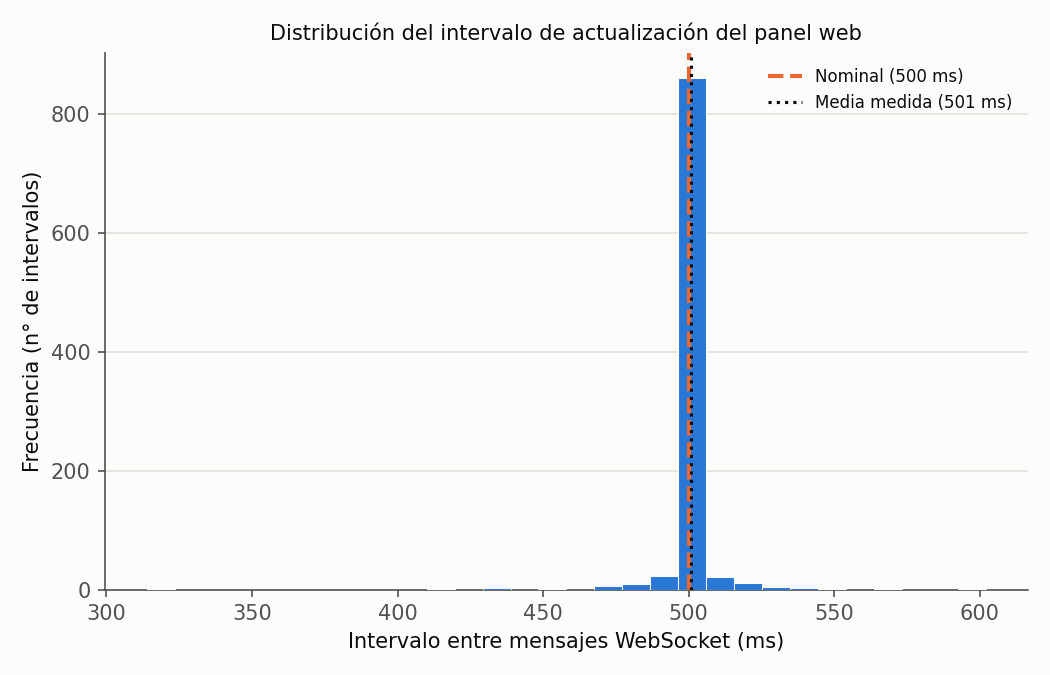
\includegraphics[width=0.8\textwidth]{Images/figura_ws_latencia.png}

	\vspace{2pt}
	{\footnotesize\textit{Nota.} Histograma de los intervalos individuales, con líneas verticales marcando el valor nominal (500\,ms) y la media medida. Se prefiere el histograma sobre otros tipos de gráfico porque la pregunta es ``qué tan dispersos están los intervalos alrededor del valor esperado'', una distribución de una sola variable continua. Elaboración propia.}
\end{figure}

\begin{table}[H]
	\centering
	\captionsetup{labelformat=simple, labelsep=newline, textfont=it, labelfont=bf, justification=raggedright, singlelinecheck=false}
	\caption{Estabilidad de la conexión WebSocket en sesión prolongada}
	\label{tab:estabilidad_ws}
	\begin{tabularx}{\textwidth}{X >{\centering\arraybackslash}p{3cm} >{\centering\arraybackslash}p{3.5cm}}
		\toprule
		\rowcolor[rgb]{0.851, 0.851, 0.851}
		Duración de la sesión & N.° de reconexiones & Observaciones \\
		\midrule
		8,1 min & 0 & Misma sesión de la Tabla~\ref{tab:latencia_panel}; sin caídas en todo el registro \\
		\bottomrule
	\end{tabularx}
	\vskip 0.15cm
	{\footnotesize \textit{Nota.} Reconexiones acumuladas reportadas por \texttt{wsStatsReport()} al cierre de la sesión. El reconector automático (\texttt{setTimeout(connectWs, 2000)}) hace que una caída puntual no requiera intervención manual; esta tabla registra cuántas veces ocurrió, no si el panel dejó de funcionar. La sesión registrada (8,1~min) es más corta que una sesión típica de uso, pero al no presentar ninguna reconexión aporta evidencia consistente con una conexión estable; ampliarla queda como posible verificación adicional.}
\end{table}

\begin{table}[H]
	\centering
	\captionsetup{labelformat=simple, labelsep=newline, textfont=it, labelfont=bf, justification=raggedright, singlelinecheck=false}
	\caption{Alcance del punto de acceso WiFi generado por el ESP32-S3}
	\label{tab:alcance_wifi}
	\begin{tabularx}{\textwidth}{>{\centering\arraybackslash}p{2.5cm} >{\centering\arraybackslash}p{3.5cm} >{\centering\arraybackslash}p{2.5cm} X}
		\toprule
		\rowcolor[rgb]{0.851, 0.851, 0.851}
		Distancia (m) & Obstáculos & ¿Conectado? & Reconectó al acercarse \\
		\midrule
		{}5 & Si (pared) & \checkmark & - \\
		{}10 & Si (pared) & \checkmark & - \\
		{}20 & Si (cuartos) & \checkmark & - \\
		\bottomrule
	\end{tabularx}
	\vskip 0.15cm
	{\footnotesize \textit{Nota.} Distancia aproximada entre el punto de acceso (ESP32-S3, dentro del vehículo) y el dispositivo que muestra el panel; agregar una fila por cada distancia probada.}
\end{table}

\subsection{Pruebas de consumo energético y modo de bajo consumo}
\label{sec:pruebas_consumo}

Esta prueba requiere medir corriente directamente sobre la placa (un multímetro o pinza en serie con la alimentación de 12\,V), algo que todavía no es posible con el prototipo actual sobre protoboard sin alterar el cableado de forma poco representativa. Queda pendiente hasta contar con la PCB ensamblada (Capítulo~5); mientras tanto, la Tabla~\ref{tab:consumo_energetico} ya incorpora la corriente \emph{teórica} de cada modo, derivada en la Sección~\ref{sec:consumo_activo} (modos activos) y la Ecuación~\eqref{eq:i12v_reposo} (\textit{deep sleep}) del Capítulo~3, y deja la columna de corriente medida en blanco para completarla en cuanto la PCB esté disponible.

\begin{table}[H]
	\centering
	\captionsetup{labelformat=simple, labelsep=newline, textfont=it, labelfont=bf, justification=raggedright, singlelinecheck=false}
	\caption{Consumo de corriente en los distintos modos de operación, teórico y medido}
	\label{tab:consumo_energetico}
	\begin{tabularx}{\textwidth}{X >{\centering\arraybackslash}p{4cm} >{\centering\arraybackslash}p{4cm}}
		\toprule
		\rowcolor[rgb]{0.851, 0.851, 0.851}
		Modo de operación & Corriente teórica (mA) & Corriente medida (mA) \\
		\midrule
		Activo, pantalla y WiFi encendidos & $\sim$52 & {}[COMPLETAR, pendiente de PCB] \\
		Activo, solo registro CAN/MicroSD & $\sim$34 & [COMPLETAR, pendiente de PCB] \\
		Deep sleep & $\sim$8 & [COMPLETAR, pendiente de PCB] \\
		\bottomrule
	\end{tabularx}
	\vspace{2mm}
	\\
	\begin{minipage}{\linewidth}
		\small
		\textit{Nota.} Corriente teórica calculada a la entrada de 12\,V (\texttt{OBD2}), sumando el aporte de cada componente a su riel nativo y convirtiendo a través de la eficiencia estimada del TPS54302 ($\sim$80\,\%), igual que en la Sección~\ref{sec:consumo} del Capítulo~3. Son estimaciones de orden de magnitud, no mediciones.
	\end{minipage}
\end{table}

\section{Resultados obtenidos}

\subsection{Resultados de la validación de la comunicación CAN}

Los resultados de la Tabla~\ref{tab:validacion_can}, obtenidos con las herramientas de la Sección~3.1, muestran una diferencia sistemática y no marginal entre ambos dispositivos en los tres indicadores medidos:

\begin{itemize}
	\item \textbf{Tramas recibidas.} El sistema propio registró 2\,936 respuestas válidas en la ventana de 5~minutos frente a 1\,712 del ELM327, un 71,5\,\% más de tramas procesadas en el mismo intervalo.
	\item \textbf{Tasa de error.} El sistema propio no presentó ninguna trama con error de bus (0 de 2\,936), mientras que el ELM327 registró 34 respuestas de error o \textit{NO DATA} sobre 1\,746 intentos clasificados, una tasa de error de $\approx 1{,}9\,\%$.
	\item \textbf{Latencia.} La latencia promedio del sistema propio (2,2~ms) fue del orden de 100 veces menor que la del ELM327 (231,4~ms).
\end{itemize}

Esta diferencia es atribuible a la arquitectura de cada dispositivo y no a una falla del ELM327: el sistema propio accede al controlador TWAI del ESP32-S3 de forma nativa, con la trama de respuesta disponible en la propia pila de firmware apenas el hardware la recibe del bus. El ELM327, en cambio, resuelve cada solicitud a través de una capa adicional de comandos AT en texto ASCII, que el propio adaptador debe traducir hacia y desde tramas CAN, y transporta el resultado por un enlace Bluetooth serie. Son dos fuentes adicionales de retardo y de posibles pérdidas de trama, ausentes en una implementación con acceso directo al controlador CAN.

Para la finalidad específica de este proyecto (adquirir parámetros del motor a alta frecuencia y con baja latencia para integrar el consumo instantáneo), el sistema desarrollado demuestra un desempeño de comunicación superior al de un adaptador comercial genérico como el ELM327, no en la precisión del cálculo de consumo en sí (que se evalúa por separado, contra el aforo real, en la Sección~\ref{sec:validacion_cuantitativa}), sino específicamente en la capa de adquisición de datos de la que depende esa precisión: una mayor tasa de muestreo efectiva y una latencia baja y estable reducen el error de integración temporal del consumo acumulado, y una tasa de error nula evita que datos corruptos o ausentes se propaguen al cálculo de \texttt{fuel\_calc.cpp}.

\subsection{Resultados de precisión del modelo Speed-Density}
\label{sec:resultados_speed_density}

La prueba estática (Sección~4.3.3) ya arrojó resultados concretos: antes de calibrar, el modelo subestimaba el caudal de aire en ralentí y 1500\,rpm ($-23{,}7\,\%$ y $-9{,}8\,\%$) y lo sobrestimaba a 2500 y 3500\,rpm ($+4{,}7\,\%$ y $+18{,}7\,\%$); tras calibrar la tabla VE con esos mismos datos, el error residual bajó a un rango de $-0{,}02\,\%$ a $+1{,}03\,\%$ (Figura~\ref{fig:post_calibracion}, Capítulo~3), una validación que, como se explicó ahí, es circular por construcción y no basta por sí sola. La Tabla~\ref{tab:validacion_dinamica} cierra ese punto con la prueba dinámica (Sección~\ref{sec:sd_prueba_dinamica}): métricas calculadas sobre una ruta real que nunca participó en la calibración.

\begin{table}[H]
	\centering
	\captionsetup{labelformat=simple, labelsep=newline, textfont=it, labelfont=bf, justification=raggedright, singlelinecheck=false}
	\caption{Métricas de validación dinámica del modelo Speed-Density (ruta real, Nissan Vanette)}
	\label{tab:validacion_dinamica}
	\begin{tabularx}{\textwidth}{X >{\centering\arraybackslash}p{2.2cm} >{\centering\arraybackslash}p{2.2cm} >{\centering\arraybackslash}p{2.2cm} >{\centering\arraybackslash}p{2.2cm}}
		\toprule
		\rowcolor[rgb]{0.851, 0.851, 0.851}
		n muestras & RMSE (g/s) & MAE (g/s) & MAPE (\%) & Pearson $r$ \\
		\midrule
		777 & 2,159 & 1,343 & 32,24 & 0,789 \\
		\bottomrule
	\end{tabularx}
	\vskip 0.15cm
	{\footnotesize \textit{Nota.} Calculado por \texttt{speed\_density\_drive\_validation.py} sobre el registro completo de \texttt{speed\_density\_drive\_log.csv} (777 muestras válidas), sin ningún dato compartido con la calibración de la Sección~4.3.3. $R^2=0{,}622$.}
\end{table}

\begin{figure}[H]
	\centering
	\caption{Distribución del error porcentual del modelo Speed-Density, ruta real (Nissan Vanette)}
	\label{fig:histograma_error_sd}
	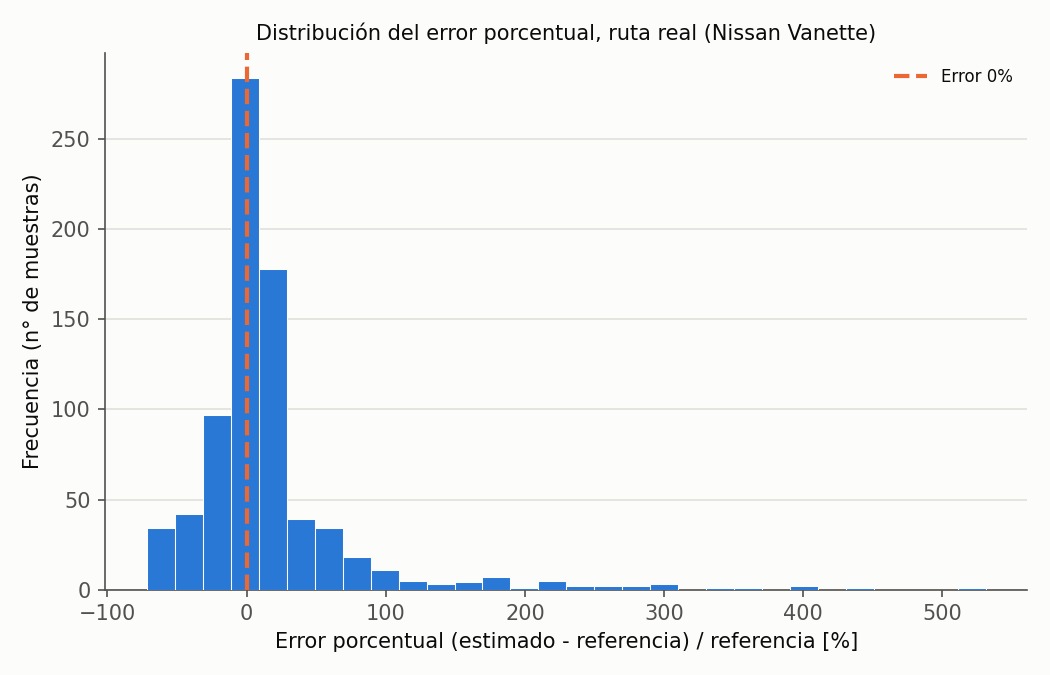
\includegraphics[width=0.8\textwidth]{Images/figura_histograma_error_dinamico.png}

	\vspace{2pt}
	{\footnotesize\textit{Nota.} Distribución del error porcentual muestra a muestra durante la ruta real; complementa la dispersión estimado-vs-referencia de la Figura~\ref{fig:dispersion_dinamica}. Elaboración propia.}
\end{figure}

La prueba dinámica confirma lo que la validación circular de la Figura~\ref{fig:post_calibracion} no podía garantizar: sobre 777 muestras de una ruta real, ajenas a la calibración, el modelo mantiene una correlación fuerte con la referencia ($r=0{,}789$, $R^2=0{,}622$) y un error absoluto moderado (RMSE $2{,}16$\,g/s, MAE $1{,}34$\,g/s sobre un rango de referencia de 2 a 16\,g/s), pero el MAPE ($32{,}2\,\%$) es considerablemente mayor que el $\pm 1\,\%$ observado en la calibración estática, la brecha esperable entre calibrar y generalizar. La Figura~\ref{fig:dispersion_dinamica} muestra por qué: la mayoría de los puntos se agrupan cerca de la recta 1:1, pero hay dispersión notable a caudal de referencia bajo (cerca de $2$\,g/s, correspondiente a ralentí y desaceleración), donde el estimado se dispara hasta $14$\,g/s en algunas muestras. El histograma de la Figura~\ref{fig:histograma_error_sd} confirma el mismo patrón: el grueso de las muestras cae cerca de $0\,\%$ de error, con una cola larga de errores porcentuales muy grandes que solo puede venir de esas condiciones de flujo bajo, donde dividir entre una referencia pequeña amplifica cualquier discrepancia absoluta modesta. Dos causas probables, no excluyentes entre sí: (1) el modelo asume un régimen cuasiestático (Sección~\ref{sec:speeddensity} del Capítulo~3), hipótesis que se degrada durante transitorios de aceleración/desaceleración reales, ausentes en la prueba estática por diseño; y (2) las cuatro lecturas de PID (RPM, MAP, IAT, MAF) se consultan de forma secuencial, no simultánea, así que en un transitorio rápido cada una corresponde a un instante ligeramente distinto. De ahí que el MAPE agregado deba leerse con cautela: está dominado por unas pocas muestras de bajo caudal, mientras que RMSE y MAE, menos sensibles a denominadores pequeños, son el indicador más representativo del error típico en conducción real.

\begin{table}[H]
	\centering
	\captionsetup{labelformat=simple, labelsep=newline, textfont=it, labelfont=bf, justification=raggedright, singlelinecheck=false}
	\caption{Validación del modelo Speed-Density en el Changan Honor}
	\label{tab:validacion_changan_sd}
	\begin{tabularx}{\textwidth}{>{\centering\arraybackslash}p{3cm} X}
		\toprule
		\rowcolor[rgb]{0.851, 0.851, 0.851}
		Vehículo & Validación disponible \\
		\midrule
		Changan Honor & No soporta el PID~0x10 (MAF), por lo que no existe una referencia directa de caudal de aire contra la cual calcular RMSE/MAE/MAPE, ni en la prueba estática ni en la dinámica (Sección~\ref{sec:ve-general} del Capítulo~3, ``Caso sin MAF''). Su exactitud se evalúa en cambio de forma indirecta, a nivel de consumo acumulado, en la Tabla~\ref{tab:comparacion_consumo_changan} (Sección~4.4.5) frente al aforo real de tanque lleno. \\
		\bottomrule
	\end{tabularx}
	\vskip 0.15cm
	{\footnotesize \textit{Nota.} A diferencia del Vanette, aquí no aplica ninguna de las métricas punto a punto de la Tabla~\ref{tab:validacion_dinamica} por ausencia de sensor de referencia, no por falta de la prueba.}
\end{table}

\subsection{Resultados de la validación del sensor MAP frente a la altitud}

Los resultados de la Tabla~\ref{tab:validacion_map_altitud} son favorables en ambos vehículos, pero no del mismo tipo de evidencia. El \textbf{Changan Honor} sí soporta el PID~0x33, así que su fila compara dos sensores reales de la propia ECU entre sí (MAP contra presión barométrica real) y da una diferencia de $0{,}0\,\%$ ($63{,}0$ frente a $63{,}0$\,kPa): una confirmación directa de que el sensor MAP reporta la presión atmosférica real de La Paz. El \textbf{Nissan Vanette}, en cambio, no soporta el PID~0x33, así que su \texttt{baro\_kpa} cae al respaldo del modelo ISA evaluado en \texttt{SITE\_ALTITUDE\_M} (Subsección~\ref{subsec:etav-altitud} del Capítulo~3); su diferencia de $-2{,}5\,\%$ ($63{,}0$ frente a $64{,}6$\,kPa) es entonces una comparación del MAP contra un \emph{modelo} de la atmósfera estándar, no contra un segundo sensor real: una validación más débil, aunque igualmente favorable. El valor ISA de $64{,}6$\,kPa es además consistente con la predicción teórica ya calculada en el Capítulo~3 ($P(3600)\approx 64{,}9$\,kPa, Ecuación~\eqref{eq:isa}), la pequeña diferencia atribuible a la altitud exacta configurada ($3640$ frente a $3600$\,m).

En ambos casos la diferencia es pequeña (menos de 2\,kPa). Esto descarta un sesgo de calibración de fábrica en el sensor MAP de cualquiera de los dos vehículos y confirma que el método speed-density parte, en ambos, de una lectura de presión correctamente calibrada para la altitud de operación, sin necesitar ningún factor de corrección adicional, como se justificó en el Capítulo~3.

\subsection{Resultados de las pruebas del panel web (WebSocket/HMI)}
\label{sec:resultados_panel_web}

Los resultados de las Tablas~\ref{tab:latencia_panel}--\ref{tab:alcance_wifi} (Changan Honor) confirman que el panel es apto para monitoreo en tiempo real: el intervalo de actualización promedió 500,0\,ms con una desviación de solo 10,0\,ms frente al periodo nominal configurado (\texttt{WS\_PUSH\_PERIOD\_MS}), sin ninguna reconexión en el registro de 8,1\,min, y sin pérdida de enlace hasta 20\,m de distancia con paredes de por medio, más que suficiente para el uso previsto, con el dispositivo dentro del mismo vehículo. Estos resultados son evidencia objetiva de la confiabilidad del panel y complementan, desde la capa de comunicación, la percepción subjetiva relevada en la encuesta de usabilidad de la Sección~\ref{sec:usabilidad_cualitativa}.

\subsection{Comparación de consumo estimado vs. consumo real}

Esta sección constituye el resultado central de la validación, ya que contrasta tres cantidades sobre nueve tramos de referencia (el corto y el medio, cada uno con 2 repeticiones completas: ida y vuelta por repetición, 4 tramos por categoría; y el largo una sola vez, sin ida/vuelta, Sección~\ref{sec:protocolo_tanque}): el consumo estimado por el sistema propio (medido de forma continua durante cada tramo), el consumo estimado por el adaptador ELM327 junto con la aplicación comercial (medido en una sesión separada e inmediatamente posterior sobre la misma ruta, por la limitación de conexión simultánea explicada en la Sección~\ref{sec:elm327_ref}), y el consumo real determinado por el método de aforo de tanque lleno a tanque lleno.

Repetir los trayectos corto y medio, y registrar ida y vuelta por separado en vez de como un solo tramo de ida-y-vuelta, no es solo para acumular más distancia: de ahí sale la \textbf{repetibilidad} del sistema propio (coeficiente de variación entre pasadas del mismo trayecto y del mismo sentido) de la Sección~\ref{sec:validacion_cuantitativa}, que de otro modo no tendría con qué calcularse; separar ida de vuelta además evita mezclar dos perfiles de tráfico/pendiente potencialmente distintos bajo un mismo número. El aforo real solo existe a nivel del \textbf{total combinado} de los nueve tramos (un único llenado de referencia cubre a todos, no se repitió por tramo, Sección~\ref{sec:protocolo_tanque}), así que la fila de ``Total'' es la única que se puede comparar directamente contra el aforo real; las filas individuales sirven para comparar el sistema propio contra el ELM327 tramo por tramo. Las Tablas~\ref{tab:comparacion_consumo_vanette} y~\ref{tab:comparacion_consumo_changan} (una por vehículo) y la Figura~\ref{fig:comparacion_consumo_grafico} presentan estos valores en forma descriptiva; el análisis estadístico formal (RMSE, MAPE, concordancia de Bland-Altman) se desarrolla por separado en la Sección~\ref{sec:validacion_cuantitativa}. Al interpretar la columna del ELM327 conviene tener presente que su comparación contra el sistema propio está sujeta a la variabilidad adicional de tratarse de una pasada distinta del mismo trayecto, y no de la misma sesión de manejo.

\begin{figure}[H]
	\centering
	\caption{Ejemplo del trayecto corto}
	\label{fig:ruta_corta}
	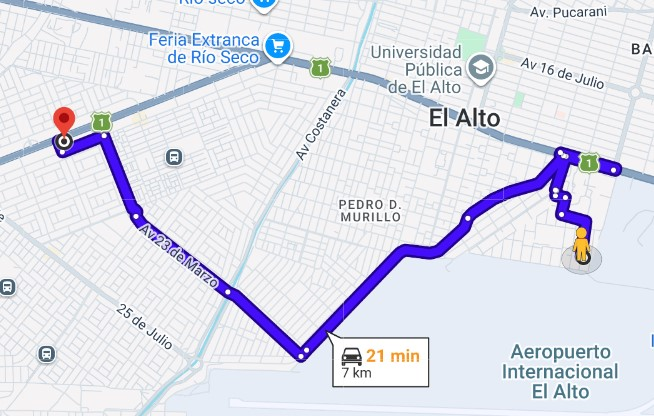
\includegraphics[width=0.8\textwidth]{Images/CORTO.jpg}
	\\
	\vspace{2pt}
	{\footnotesize\textit{Nota.} Recorrido de referencia del trayecto corto, con 2 repeticiones completas (ida y vuelta cada una, Tablas~\ref{tab:comparacion_consumo_vanette}/\ref{tab:comparacion_consumo_changan}); la ruta real puede variar levemente entre repeticiones. Elaboración propia.}
\end{figure}

\begin{figure}[H]
	\centering
	\caption{Ejemplo del trayecto medio}
	\label{fig:ruta_media}
	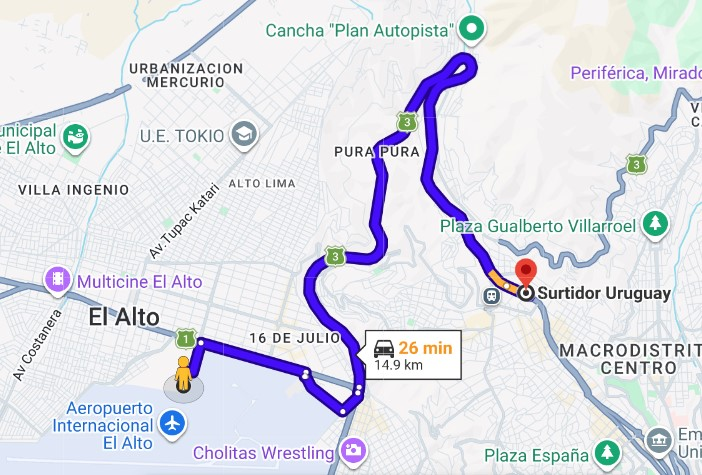
\includegraphics[width=0.8\textwidth]{Images/MEDIA.jpg}
	\\
	\vspace{2pt}
	{\footnotesize\textit{Nota.} Recorrido de referencia del trayecto medio, con 2 repeticiones completas (ida y vuelta cada una). Elaboración propia.}
\end{figure}

\begin{figure}[H]
	\centering
	\caption{Trayecto del viaje largo}
	\label{fig:ruta_larga}
	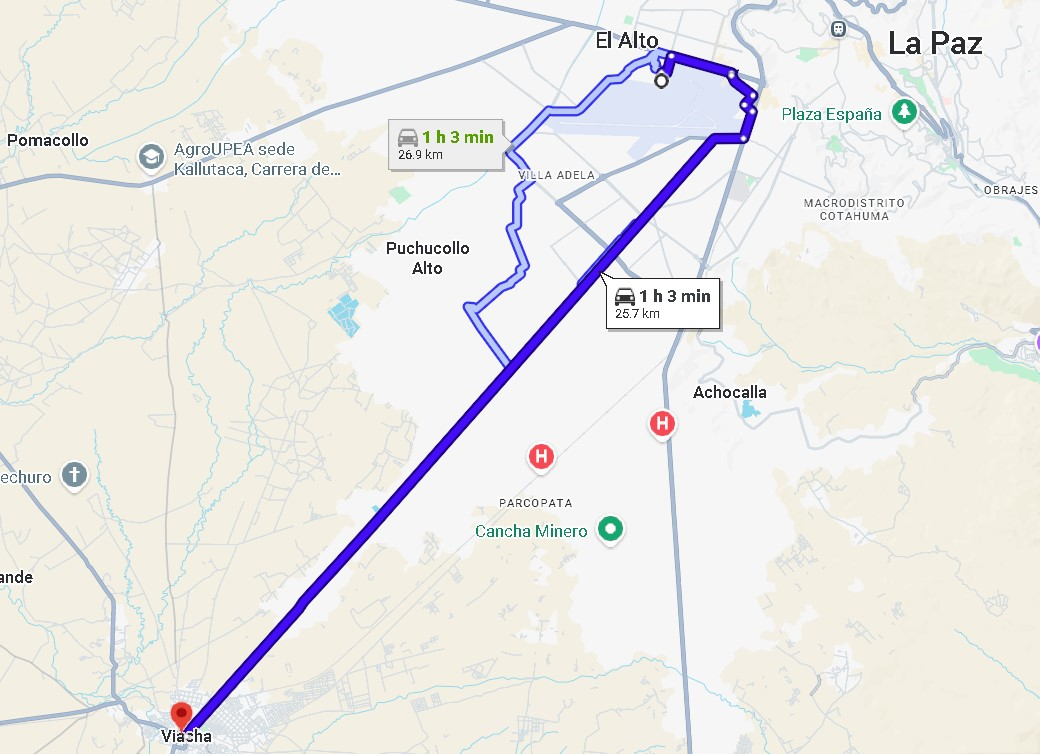
\includegraphics[width=0.8\textwidth]{Images/LARGO.jpg}
	\\
	\vspace{2pt}
	{\footnotesize\textit{Nota.} Recorrido único (sin repetición) del trayecto largo. Elaboración propia.}
\end{figure}

Las tres rutas de la Figura~\ref{fig:ruta_corta}--\ref{fig:ruta_larga} se recorrieron con \textbf{ambos vehículos} por separado, cada uno con su propio par de llenados de referencia; la Tabla~\ref{tab:comparacion_consumo_vanette} y la Tabla~\ref{tab:comparacion_consumo_changan} presentan los resultados de cada uno.

\begin{table}[H]
	\centering
	\captionsetup{labelformat=simple, labelsep=newline, textfont=it, labelfont=bf, justification=raggedright, singlelinecheck=false}
	\caption{Comparación de consumo de combustible entre el sistema propuesto, la referencia comercial y el consumo real, por trayecto (Nissan Vanette)}
	\label{tab:comparacion_consumo_vanette}
	\begin{tabularx}{\textwidth}{X >{\centering\arraybackslash}p{2.3cm} >{\centering\arraybackslash}p{2.8cm} >{\centering\arraybackslash}p{2.8cm} >{\centering\arraybackslash}p{2.8cm}}
		\toprule
		\rowcolor[rgb]{0.851, 0.851, 0.851}
		Trayecto & Distancia (km) & Sistema propuesto (L) & ELM327 + app (L)$^{a}$ & Real, tanque lleno (L) \\
		\midrule
		Viaje corto 1 (ida) & {}5,72 & 0,52 & 0,50 & --- \\
		Viaje corto 1 (vuelta) & 5,53 & 0,46 & 0,49 & --- \\
		Viaje corto 2 (ida) & 10,56 & 1,12 & 1,15 & --- \\
		Viaje corto 2 (vuelta) & 10,49 & 1,24 & 1,28 & --- \\
		Viaje medio 1 (ida) & 14,31 & 1,23 & 1,22 & --- \\
		Viaje medio 1 (vuelta) & 15,10 & 1,57 & 1,61 & --- \\
		Viaje medio 2 (ida) & 18,01 & 1,66 & 1,68 & --- \\
		Viaje medio 2 (vuelta) & 18,24 & 1,86 & 1,89 & --- \\
		Viaje largo & 26,3 & 2,43 & 2,44 & --- \\
		\midrule
		\textbf{Total (suma de los 9)} & \textbf{124,26} & \textbf{12,09} & \textbf{12,26} & \textbf{12,96} \\
		\bottomrule
	\end{tabularx}
	\vspace{2mm}
	\\
	\begin{minipage}{\linewidth}
		\small
		\textit{Nota.} Prototipo frente a herramienta comercial y reabastecimiento real. $^{a}$Sesión separada, misma ruta (Sección~\ref{sec:elm327_ref}). Aforo real solo en el total (Sección~\ref{sec:protocolo_tanque}). Viajes medio y largo: litros = gasto en Bs / 6,96\,Bs/L (\texttt{FUEL\_PRICE\_BS\_PER\_L}).
	\end{minipage}
\end{table}

\begin{table}[H]
	\centering
	\captionsetup{labelformat=simple, labelsep=newline, textfont=it, labelfont=bf, justification=raggedright, singlelinecheck=false}
	\caption{Comparación de consumo de combustible entre el sistema propuesto, la referencia comercial y el consumo real, por trayecto (Changan Honor)}
	\label{tab:comparacion_consumo_changan}
	\begin{tabularx}{\textwidth}{X >{\centering\arraybackslash}p{2.3cm} >{\centering\arraybackslash}p{2.8cm} >{\centering\arraybackslash}p{2.8cm} >{\centering\arraybackslash}p{2.8cm}}
		\toprule
		\rowcolor[rgb]{0.851, 0.851, 0.851}
		Trayecto & Distancia (km) & Sistema propuesto (L) & ELM327 + app (L)$^{a}$ & Real, tanque lleno (L) \\
		\midrule
		Viaje corto 1 (ida) & {}6,28 & 0,52 & 0,53 & --- \\
		Viaje corto 1 (vuelta) & 6,14 & 0.58 & 0,57 & --- \\
		Viaje corto 2 (ida) & 6,74 & 0,60 & 0,56 & --- \\
		Viaje corto 2 (vuelta) & 4.02 & 0,40 & 0,42 & --- \\
		Viaje medio 1 (ida) & 14,25 & 1,00 & 0,99 & --- \\
		Viaje medio 1 (vuelta) & 15,04 & 1,39 & 1,31 & --- \\
		Viaje medio 2 (ida) & 18,01 & 1,30 & 1,33 & --- \\
		Viaje medio 2 (vuelta) & 17,78 & 1,71 & 1,68 & --- \\
		Viaje largo & 25,99 & 1,839 & 1,825 & --- \\
		\midrule
		\textbf{Total (suma de los 9)} & \textbf{114,25} & \textbf{9,34} & \textbf{9,21} & \textbf{9,07} \\
		\bottomrule
	\end{tabularx}
	\vspace{2mm}
	\\
	\begin{minipage}{\linewidth}
		\small
		\textit{Nota.} Igual estructura que la Tabla~\ref{tab:comparacion_consumo_vanette}. Sin PID~0x10, ``sistema propuesto'' corre en Speed-Density puro; esta tabla es la validación aguas abajo de la Tabla~\ref{tab:validacion_changan_sd}. $^{a}$Ídem nota anterior.
	\end{minipage}
\end{table}

\begin{figure}[H]
	\centering
	\caption{Comparación gráfica del consumo de combustible por trayecto y vehículo según los tres métodos evaluados}
	\label{fig:comparacion_consumo_grafico}
	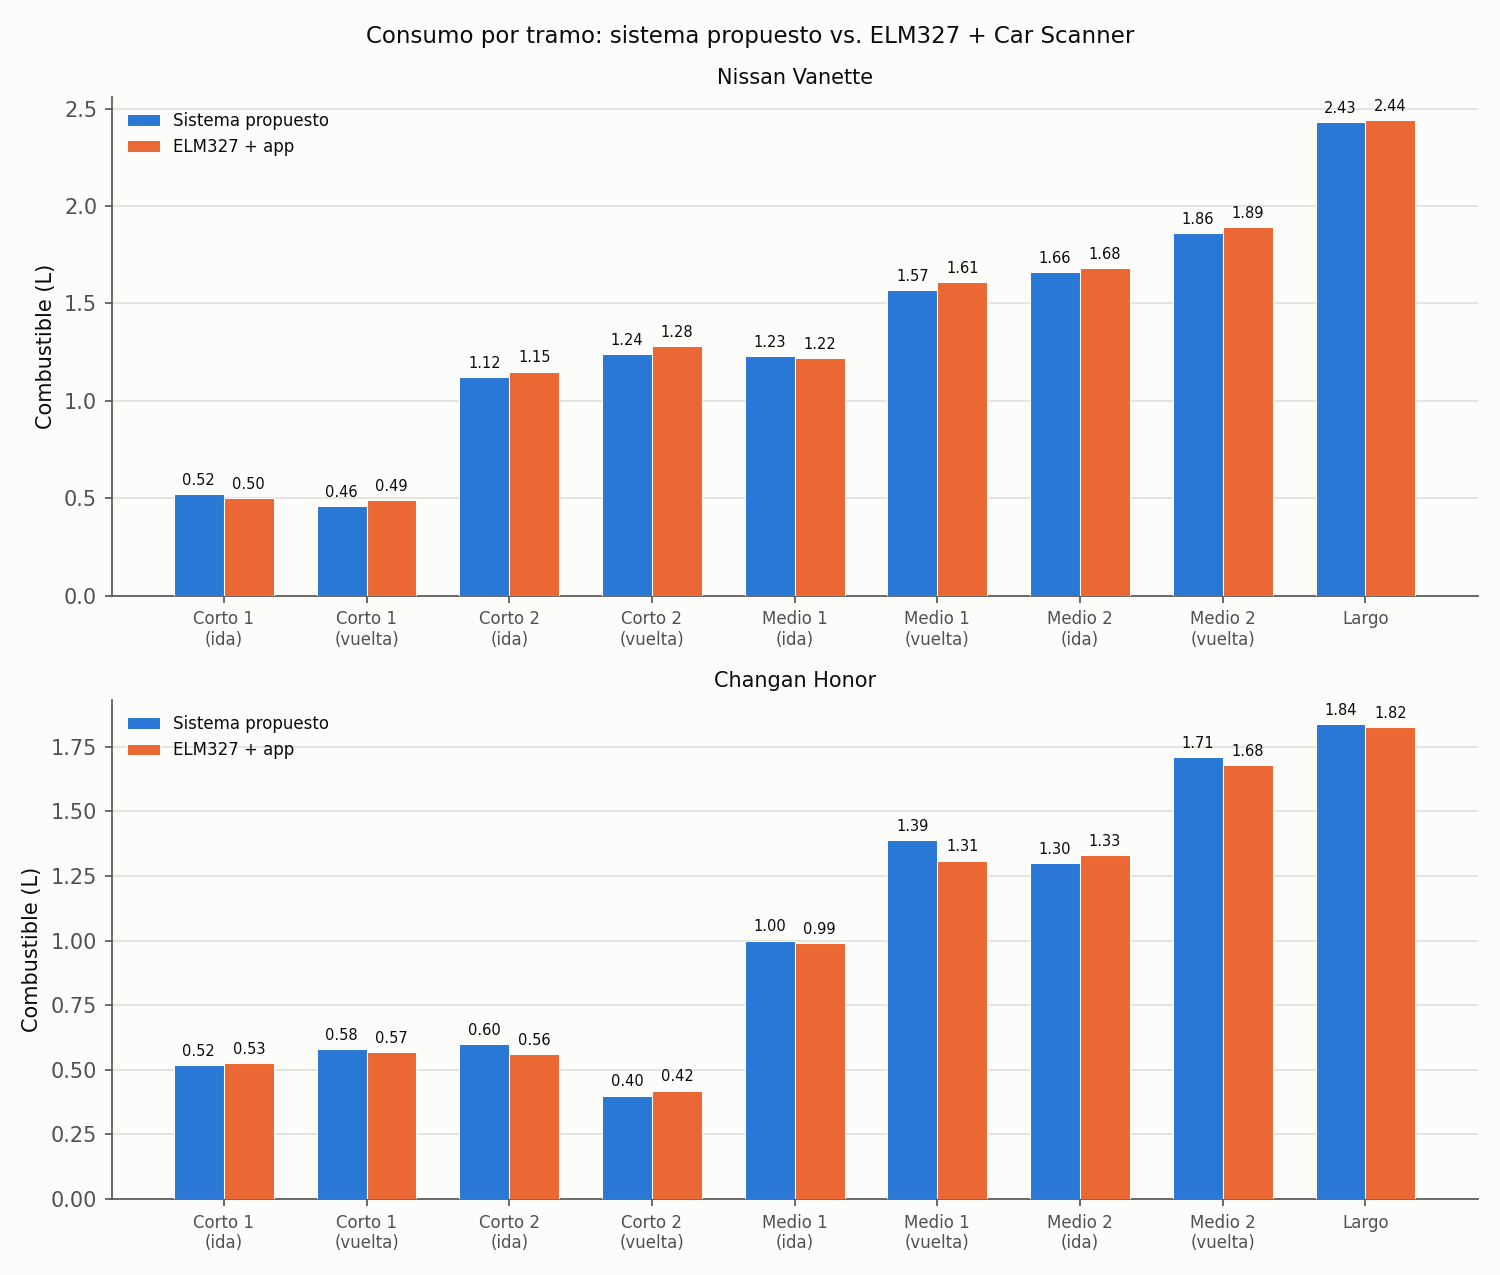
\includegraphics[width=\textwidth]{Images/figura_comparacion_consumo.png}

	\vspace{2pt}
	{\footnotesize\textit{Nota.} Comparativa del volumen de combustible estimado frente a las lecturas obtenidas por cada método, tramo por tramo, para cada vehículo. Elaboración propia.}
\end{figure}

Con los nueve tramos completos en ambos vehículos, el acuerdo entre el sistema propio y el ELM327 + Car Scanner vuelve a ser bueno en el total combinado ($-1{,}4\,\%$ en el Vanette: $12{,}090$ frente a $12{,}260$\,L en $124{,}26$\,km; y $+1{,}4\,\%$ en el Changan: $9{,}338$ frente a $9{,}212$\,L en $114{,}25$\,km), aunque, a diferencia de la comparación con solo tres trayectos, ahora el error por tramo individual oscila en ambos sentidos y con más dispersión: de $-6{,}1\,\%$ a $+4{,}0\,\%$ en el Vanette, y de $-4{,}8\,\%$ a $+7{,}1\,\%$ en el Changan, sin que el signo se mantenga constante ni siquiera entre ida y vuelta del mismo trayecto. Esto es consistente con lo ya discutido en la Figura~\ref{fig:ve_consumo_impacto}: el error por tramo depende de la mezcla de regímenes de motor de ese tramo en particular, no es una propiedad fija del ``trayecto corto'' o ``trayecto medio'' como categoría.

Al tener ahora dos repeticiones de cada categoría, se puede estimar por primera vez la \textbf{repetibilidad} del sistema propio (Sección~\ref{sec:validacion_cuantitativa}): el coeficiente de variación del consumo normalizado (L/100\,km) entre las 4 mediciones de cada categoría es de $13{,}6\,\%$ (corto) y $7{,}6\,\%$ (medio) en el Vanette, y de $6{,}9\,\%$ (corto) y $14{,}1\,\%$ (medio) en el Changan. Esta variabilidad, de un solo dígito alto a poco más de $13\,\%$, es del orden de magnitud esperable para conducción real en tráfico urbano de La Paz, donde el mismo trayecto nominal rara vez se recorre dos veces en condiciones idénticas (semáforos, tráfico, pendiente efectiva según el sentido); no debe leerse como ruido propio del sistema de medición, ya que la Tabla~\ref{tab:validacion_dinamica} ya mostró que el modelo, sobre las mismas condiciones de manejo, correlaciona fuertemente con el MAF real ($r=0{,}789$).

\subsubsection*{De dónde viene la diferencia: impacto de la curva VE en el consumo}

Las Tablas~\ref{tab:speed_density_resultados} y~\ref{tab:validacion_dinamica} ya mostraron que la tabla VE calibrada no es igual de precisa en todo el rango de régimen; lo que no muestran es cuánto vale eso en litros. La Figura~\ref{fig:ve_consumo_impacto}, generada por \texttt{CODIGOS/ve\_consumo\_impacto.py} sobre el mismo registro de la prueba dinámica (Sección~\ref{sec:sd_prueba_dinamica}), conecta ambas cosas: agrupa las muestras por bin de RPM y, en cada uno, calcula tanto el consumo instantáneo que resulta de la VE calibrada como el que resultaría del MAF real, expresando la diferencia directamente en L/100km en vez de en g/s de aire.

\begin{figure}[H]
	\centering
	\caption{Curva VE calibrada y su impacto en el consumo estimado, por bin de RPM (ruta real, Nissan Vanette)}
	\label{fig:ve_consumo_impacto}
	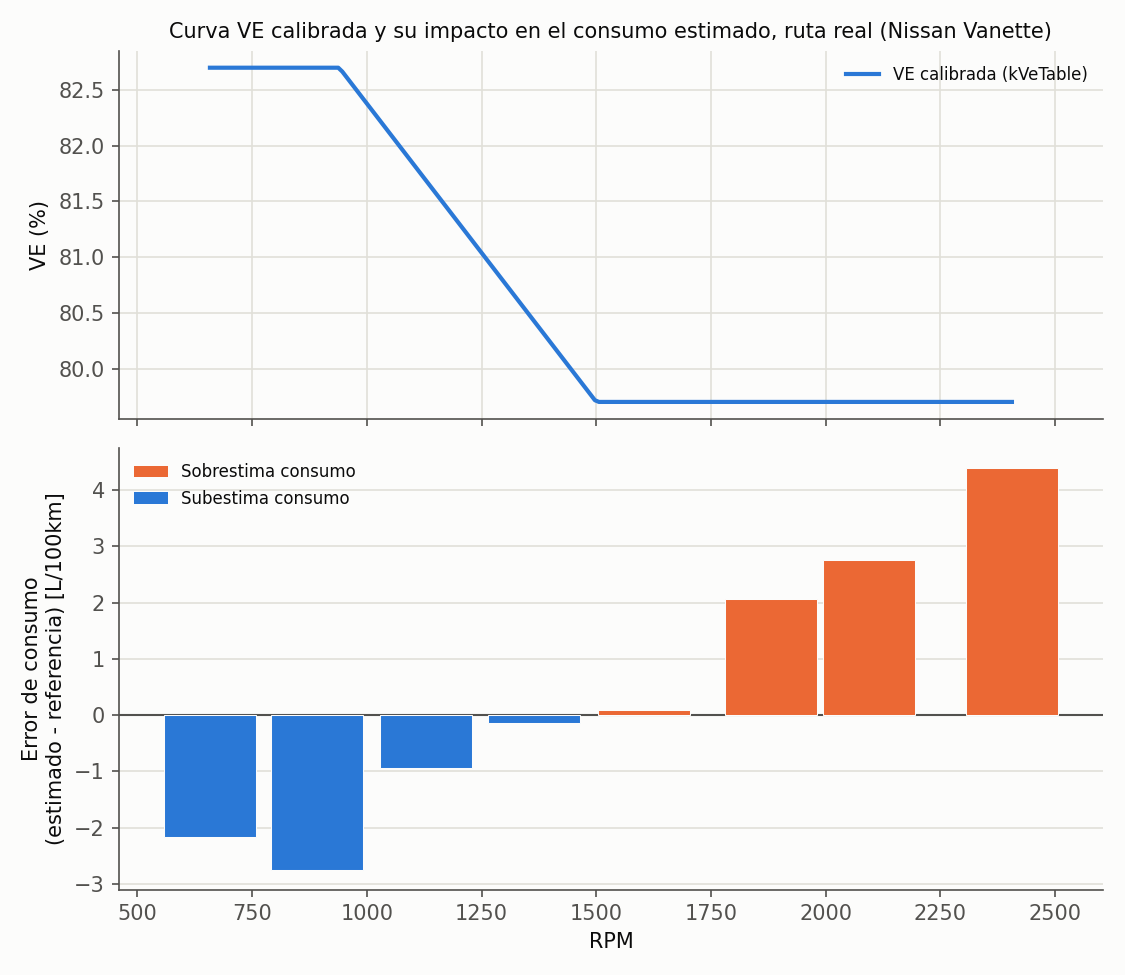
\includegraphics[width=0.85\textwidth]{Images/figura_ve_consumo_impacto.png}

	\vspace{2pt}
	{\footnotesize\textit{Nota.} Panel superior: curva VE calibrada (\texttt{kVeTable}) en el rango de RPM cubierto por la ruta. Panel inferior: error de consumo promedio por bin de RPM (estimado $-$ referencia), con barras coloreadas por signo. Ambos paneles comparten el eje de RPM para leer directamente en qué régimen se origina cada tramo de la diferencia. Elaboración propia.}
\end{figure}

El patrón es claro y consistente con la Figura~\ref{fig:histograma_error_sd}: por debajo de $\sim$1500\,rpm el sistema \textbf{subestima} el consumo (hasta $-2{,}7$\,L/100km en el bin de $\sim$890\,rpm), y por encima de $\sim$1600\,rpm lo \textbf{sobrestima}, con una brecha creciente que llega a $+4{,}4$\,L/100km cerca de $2400$\,rpm. Esto es consecuencia directa de la forma de la tabla VE calibrada (Tabla~\ref{tab:ve_calibracion}, Capítulo~3): con solo cuatro puntos calibrados contra régimen sostenido y sin datos por encima de $3500$\,rpm, la curva no captura del todo la variación real de la eficiencia volumétrica del motor durante los transitorios de una ruta: la misma limitación ya discutida en la Sección~\ref{sec:sd_prueba_dinamica}. En términos prácticos, esto explica por qué el error total de un trayecto del Vanette (Tabla~\ref{tab:comparacion_consumo_vanette}) no es simplemente la suma de errores aleatorios: depende de qué proporción del viaje se pasó en cada rango de régimen, de modo que una ruta con más tramos por encima de $1600$\,rpm tenderá a mostrar una sobrestimación neta mayor que una de manejo predominantemente urbano a bajas revoluciones.

\subsection{Desempeño del sistema en condiciones reales de conducción}

Con los nueve tramos ya medidos en ambos vehículos (Tablas~\ref{tab:comparacion_consumo_vanette} y~\ref{tab:comparacion_consumo_changan}), el sistema propio se mantiene cerca del ELM327 + Car Scanner en el total combinado: $-1{,}4\,\%$ en el Vanette, $+1{,}4\,\%$ en el Changan (Sección~\ref{sec:validacion_cuantitativa} desarrolla las métricas formales sobre estos mismos datos). Vale la pena notar la aparente contradicción con el $32\,\%$ de MAPE de la Sección~\ref{sec:resultados_speed_density}: esas cifras no son incompatibles, sino que miden cosas distintas. El MAPE se calcula muestra a muestra, así que un error grande y de signo variable en cada instante (Figura~\ref{fig:ve_consumo_impacto}) puede compensarse casi por completo al integrarlo en litros a lo largo de todo un trayecto, si el tiempo pasado sobrestimando y subestimando es comparable. En otras palabras: el modelo es menos preciso instante a instante de lo que sugiere el litraje total de un viaje, una distinción relevante para cualquier uso que dependa de la lectura instantánea (por ejemplo, retroalimentar el estilo de conducción en tiempo real) y no solo del acumulado al final del trayecto.

Los tramos cortos fueron viajes de no más de 15 minutos circulando en la ciudad de El Alto: el terreno fue en general plano, con la excepción del tráfico denso en los distintos puntos céntricos recorridos. Los tramos medios cubrieron mayor distancia y se realizaron por dos zonas distintas de la urbe paceña, cada una con su propia condición particular. Uno de ellos aprovechó la autopista La Paz-El Alto, donde se observa una asimetría clara entre ida y vuelta: en la bajada el acelerador no se pisa de forma continua, lo que se refleja en el menor consumo registrado por el sistema (Medio~1 ida, $8{,}60$\,L/100\,km, Tabla~\ref{tab:comparacion_consumo_vanette}); en la subida de vuelta, en cambio, el acelerador se mantiene pisado por más tiempo, y el consumo sube de forma correspondiente ($10{,}40$\,L/100\,km). El otro tramo medio se realizó por las avenidas principales de la ciudad de La Paz, esta vez con mayor peso a bordo del vehículo, factor que también influye en el consumo. En todos los tramos cortos y medios la temperatura ambiente fue fría, ya que las pruebas se realizaron de madrugada o por la noche.

En el viaje largo a Viacha, el sistema reaccionó de forma más lenta de lo esperado al inicio del trayecto, pero se estabilizó conforme avanzó el recorrido, resultado consistente con la calibración de la curva de eficiencia volumétrica del Nissan Vanette (Sección~\ref{sec:calibracion_speed_density}). Comparado con el Changan Honor, se esperaba, y se observó en el total combinado (Tablas~\ref{tab:comparacion_consumo_vanette}/\ref{tab:comparacion_consumo_changan}), un consumo menor en el Changan, coherente con su cilindrada más pequeña frente a la del Vanette.

\section{Validación del sistema}
\label{sec:validacion_cuantitativa}

\subsection{Validación cuantitativa (error porcentual y métricas estadísticas)}

Tomando como insumo los mismos trayectos ya presentados de forma descriptiva en las Tablas~\ref{tab:comparacion_consumo_vanette} y~\ref{tab:comparacion_consumo_changan} (Sección~4.4), se recomienda calcular, para cada conjunto de datos comparado (sistema propio frente a ELM327 y app, y sistema propio frente al consumo real de tanque lleno), las siguientes métricas (con las herramientas y fórmulas ya detalladas en la Sección~\ref{sec:herramientas_analisis}):

\begin{itemize}
	\item \textbf{Error porcentual relativo}, punto a punto, definido como:
	\begin{equation}
		\text{Error}_{\%} = \frac{|V_{\text{estimado}} - V_{\text{referencia}}|}{V_{\text{referencia}}} \times 100
		\label{eq:error_porcentual_relativo}
	\end{equation}
	\item \textbf{Error cuadrático medio (RMSE)} y \textbf{error absoluto medio (MAE)}, que expresan la magnitud típica del error en las mismas unidades que la variable medida (litros o litros por cada 100\,km), sobre los $n$ tramos comparados:
	\begin{equation}
		\text{RMSE} = \sqrt{\frac{1}{n}\sum_{i=1}^{n}\left(V_{\text{estimado},i} - V_{\text{referencia},i}\right)^2}
		\label{eq:rmse}
	\end{equation}
	\begin{equation}
		\text{MAE} = \frac{1}{n}\sum_{i=1}^{n}\left|V_{\text{estimado},i} - V_{\text{referencia},i}\right|
		\label{eq:mae}
	\end{equation}
	\item \textbf{Error porcentual absoluto medio (MAPE)}, útil para comparar el desempeño entre trayectos de distinta longitud; es el promedio del error porcentual relativo (Ecuación~\ref{eq:error_porcentual_relativo}) sobre los $n$ tramos:
	\begin{equation}
		\text{MAPE} = \frac{1}{n}\sum_{i=1}^{n}\frac{\left|V_{\text{estimado},i} - V_{\text{referencia},i}\right|}{V_{\text{referencia},i}} \times 100
		\label{eq:mape}
	\end{equation}
	\item \textbf{Coeficiente de correlación de Pearson} y \textbf{coeficiente de determinación ($R^2$)} de una regresión lineal entre los valores estimados y los de referencia, que indican qué tan bien se explica la variación de un método a partir del otro:
	\begin{equation}
		r = \frac{\displaystyle\sum_{i=1}^{n}\left(V_{\text{estimado},i}-\overline{V}_{\text{estimado}}\right)\left(V_{\text{referencia},i}-\overline{V}_{\text{referencia}}\right)}{\sqrt{\displaystyle\sum_{i=1}^{n}\left(V_{\text{estimado},i}-\overline{V}_{\text{estimado}}\right)^2}\ \sqrt{\displaystyle\sum_{i=1}^{n}\left(V_{\text{referencia},i}-\overline{V}_{\text{referencia}}\right)^2}}
		\label{eq:pearson_r}
	\end{equation}
	con $R^2 = r^2$ para el caso de una regresión lineal simple entre las dos series.
	\item \textbf{Análisis de concordancia de Bland-Altman}, recomendado específicamente para comparar dos métodos de medición que estiman una misma magnitud, como es el caso del sistema propuesto frente al adaptador ELM327 con su aplicación comercial. Este método grafica la diferencia entre ambas mediciones contra su promedio, y permite estimar el sesgo medio y los límites de concordancia, evidenciando si existe un sesgo sistemático entre los dos sistemas y no solo una correlación:
	\begin{align}
		d_i &= V_{\text{estimado},i} - V_{\text{referencia},i} \label{eq:ba_diferencia}\\
		\overline{d} &= \frac{1}{n}\sum_{i=1}^{n} d_i \qquad \text{(sesgo medio)} \label{eq:ba_sesgo}\\
		\text{LoA} &= \overline{d} \pm 1{,}96\, s_d \label{eq:ba_loa}
	\end{align}
	donde $s_d$ es la desviación estándar (muestral) de las diferencias $d_i$.
	\item \textbf{Repetibilidad}, expresada como el coeficiente de variación del sistema propio al repetir el mismo trayecto varias veces bajo condiciones similares; esto separa el error atribuible al método de estimación del error atribuible a la variabilidad de la conducción. Se calcula sobre las $n=4$ mediciones de consumo normalizado (L/100\,km) de una misma categoría de trayecto (ida y vuelta $\times$ 2 repeticiones) y vehículo:
	\begin{equation}
		\text{CV} = \frac{s}{\overline{x}} \times 100
		\label{eq:cv_repetibilidad}
	\end{equation}
	con $\overline{x}$ la media y $s$ la desviación estándar de esas $n=4$ mediciones.
\end{itemize}

La Tabla~\ref{tab:metricas_validacion} propone el formato de resumen de estas métricas.

\begin{table}[H]
	\centering
	\small
	\captionsetup{labelformat=simple, labelsep=newline, textfont=it, labelfont=bf, justification=raggedright, singlelinecheck=false}
	\caption{Resumen de métricas de validación cuantitativa}
	\label{tab:metricas_validacion}
	\begin{tabularx}{\textwidth}{X >{\centering\arraybackslash}p{3.2cm} >{\centering\arraybackslash}p{3.2cm}}
		\toprule
		\rowcolor[rgb]{0.851, 0.851, 0.851}
		Métrica & Sistema propio vs. ELM327+app & Sistema propio vs. tanque lleno \\
		\midrule
		RMSE (L) & 0,0312 & 0,64$^{c}$ \\
		MAE (L) & 0,0262 & 0,57$^{c}$ \\
		MAPE (\%) & 2,75 & 4,84$^{c}$ \\
		$R^2$ & 0,9971 & ---$^{c}$ \\
		Sesgo medio, Bland-Altman (L) & $-0,0024$ & ---$^{c}$ \\
		Límites de concordancia (L) & $[-0,0635,\ 0,0586]$ & ---$^{c}$ \\
		Repetibilidad$^{b}$ (CV, \%): Vanette corto & 13,6 & --- \\
		Repetibilidad$^{b}$ (CV, \%): Vanette medio & 7,6 & --- \\
		Repetibilidad$^{b}$ (CV, \%): Changan corto & 6,9 & --- \\
		Repetibilidad$^{b}$ (CV, \%): Changan medio & 14,1 & --- \\
		\bottomrule
	\end{tabularx}
	\vspace{2mm}
	\\
	\begin{minipage}{\linewidth}
		\small
		\textit{Nota.} Estadísticos de precisión, error global y concordancia evaluados para validar el ajuste numérico del modelo desarrollado frente a las referencias. Sistema propio vs. ELM327+app calculado sobre los 18 tramos combinados de ambos vehículos (Tablas~\ref{tab:comparacion_consumo_vanette}/\ref{tab:comparacion_consumo_changan}). $^{b}$La repetibilidad no es una comparación \textit{vs.}\ una referencia externa, sino la variabilidad del propio sistema (coeficiente de variación del consumo en L/100\,km) entre las 4 mediciones de cada categoría de trayecto por vehículo; se deja en la primera columna por consistencia visual con el resto de filas, y el guion en la segunda porque no aplica una comparación contra el tanque lleno. $^{c}$Sistema propio vs. tanque lleno tiene $n=2$ (el total del Vanette y el del Changan, Tablas~\ref{tab:comparacion_consumo_vanette}/\ref{tab:comparacion_consumo_changan}: único nivel en el que existe aforo real, Sección~\ref{sec:protocolo_tanque}); RMSE, MAE y MAPE se reportan igual sobre esos dos puntos, pero deben leerse como una referencia gruesa y no como una estimación estadísticamente robusta. $R^2$ y el análisis de Bland-Altman no se reportan en esta columna porque con $n=2$ el coeficiente de correlación es trivialmente $\pm 1$ (una recta pasa exactamente por cualquier par de puntos) y no refleja una bondad de ajuste real.
	\end{minipage}
\end{table}

\subsection{Validación cualitativa (usabilidad de la interfaz y confiabilidad)}
\label{sec:usabilidad_cualitativa}

Se recomienda complementar la validación numérica con una evaluación cualitativa breve de usabilidad, por ejemplo mediante una escala de Likert de 5 puntos aplicada a un pequeño grupo de usuarios (conductores de los vehículos de prueba o compañeros del programa), sobre aspectos como la claridad de la información mostrada en la pantalla OLED, la facilidad de acceso al panel web, y la percepción general de confiabilidad del dispositivo durante el uso cotidiano. Esta encuesta mide la \emph{percepción} del usuario; como contraparte objetiva de la afirmación ``confiaría en el valor mostrado'', la Sección~\ref{sec:resultados_panel_web} ya reporta datos medidos de la estabilidad y latencia reales de la conexión con el panel.

\begin{table}[H]
	\centering
	\captionsetup{labelformat=simple, labelsep=newline, textfont=it, labelfont=bf, justification=raggedright, singlelinecheck=false}
	\caption{Formato de encuesta de usabilidad (escala de Likert, 1 = muy en desacuerdo, 5 = muy de acuerdo)}
	\label{tab:usabilidad}
	\begin{tabularx}{\textwidth}{X *{5}{>{\centering\arraybackslash}p{1cm}}}
		\toprule
		\rowcolor[rgb]{0.851, 0.851, 0.851}
		Afirmación & 1 & 2 & 3 & 4 & 5 \\
		\midrule
		La información en la pantalla OLED es clara y legible & & &\checkmark & & \\
		El panel web es fácil de interpretar & & &\checkmark & & \\
		El dispositivo no interfiere con la conducción & & & & & \checkmark\\
		Confiaría en el valor de consumo mostrado & & & &\checkmark & \\
		\bottomrule
	\end{tabularx}
	\vspace{2mm}
	\\
	\begin{minipage}{\linewidth}
		\small
		\textit{Nota.} Cuestionario cualitativo diseñado para medir la percepción de usuario en aspectos de legibilidad, ergonomía e interfaz del prototipo desarrollado.
	\end{minipage}
\end{table}

\subsection{Discusión de resultados frente a los objetivos del proyecto}

Retomando los seis objetivos específicos planteados en el Capítulo~1, a continuación se discute, uno por uno, en qué medida los resultados de este capítulo los satisfacen:

\begin{itemize}
	\item \textbf{Determinar los parámetros del sistema OBD-II disponibles.} Se cumple: la Tabla~\ref{tab:pids_verificacion} confirma que ambos vehículos exponen RPM (\texttt{0x0C}) y velocidad (\texttt{0x0D}), pero difieren justo en el parámetro crítico del modelo: el Nissan Vanette reporta MAF (\texttt{0x10}) y el Changan Honor no. Esta asimetría, lejos de ser un obstáculo, es la que motivó desarrollar la ruta alternativa sin MAF (VE genérica y STFT/LTFT, Sección~\ref{sec:ve-general} del Capítulo~3) que exige implícitamente el objetivo al hablar de MAF \emph{y/o} MAP.

	\item \textbf{Desarrollar un modelo matemático de estimación basado en la relación aire-combustible.} Cumplido mediante el modelo Speed-Density calibrado en el Capítulo~3 y puesto a prueba en este: la calibración de la tabla VE con datos reales del Vanette (Sección~\ref{sec:calibracion_speed_density}) y su aplicación en la prueba dinámica de ruta real (Tabla~\ref{tab:validacion_dinamica}, $r=0{,}789$) muestran que el modelo captura la tendencia del caudal de aire real, aunque con una dispersión instantánea considerable (MAPE del $32\,\%$ punto a punto) que debe leerse como una limitación del modelo en sí, no solo de su calibración.

	\item \textbf{Adquirir y registrar datos del motor mediante OBD-II.} Este objetivo se cumple: el firmware adquiere y registra RPM, MAP o MAF, IAT y velocidad en cada ciclo, con una tasa de integridad de registro en MicroSD del $100\,\%$ (0 archivos corruptos en las tres sesiones de la Tabla~\ref{tab:validacion_microsd}, incluida una prueba deliberada de corte abrupto de energía).

	\item \textbf{Diseñar un sistema embebido de adquisición para validar el modelo.} Cumplido también: el prototipo basado en ESP32-S3 (Capítulo~3) fue el instrumento con el que se generaron todos los datos de este capítulo, desde la validación estática (Tabla~\ref{tab:speed_density_resultados}) hasta los nueve tramos de ruta real (Tablas~\ref{tab:comparacion_consumo_vanette}/\ref{tab:comparacion_consumo_changan}).

	\item \textbf{Diseñar e implementar una plataforma telemétrica IoT.} Cumplido de forma parcial. El ESP32-S3 sí actúa como servidor local, transmite la telemetría por WebSocket con latencia estable ($500{,}0 \pm 10{,}0$\,ms sobre 945 muestras, Tabla~\ref{tab:latencia_panel}) y sin reconexiones en la sesión prolongada registrada (Tabla~\ref{tab:estabilidad_ws}), y el punto de acceso WiFi se mantuvo conectado hasta los $20$\,m, la mayor distancia probada (Tabla~\ref{tab:alcance_wifi}), suficiente para el caso de uso dentro de un vehículo. Sin embargo, el objetivo específico planteaba explícitamente el almacenamiento en una \emph{base de datos estructurada}; lo efectivamente implementado es un registro en archivos CSV sobre MicroSD, sin una base de datos relacional o documental de por medio. Esta es una limitación real frente al objetivo original, que queda como trabajo futuro (por ejemplo, una capa de sincronización periódica del CSV hacia una base de datos en el servidor local o en la nube).

	\item \textbf{Evaluar el sistema integral bajo condiciones reales.} Cumplido con matices. El acuerdo global frente al ELM327 + Car Scanner es bueno sobre los nueve tramos ($-1{,}4\,\%$ Vanette, $+1{,}4\,\%$ Changan) y, frente al aforo real de tanque lleno, se mantiene en el mismo orden de magnitud (MAPE $\approx 4{,}8\,\%$, Sección~\ref{sec:validacion_cuantitativa}); pero dos limitaciones deben señalarse explícitamente. Primero, el tamaño de muestra es reducido —nueve tramos por vehículo y un único par de vehículos—, insuficiente para generalizar sin pruebas adicionales al resto de la flota de transporte público de La Paz. Segundo, los dos vehículos de prueba no se comportaron de forma equivalente frente al sistema: el Changan Honor, al no soportar el PID de MAF, solo pudo validarse de forma indirecta (a nivel de consumo acumulado) y no cuenta con la validación dinámica punto a punto que sí tiene el Vanette (Tabla~\ref{tab:validacion_dinamica}). Esta asimetría entre vehículos es en sí misma un hallazgo relevante, y amerita, como trabajo futuro, repetir la prueba dinámica en un vehículo adicional con sensor MAF para confirmar que el patrón de error observado no es específico de un solo motor.
\end{itemize}

Como cierre metodológico, conviene recordar que el modelo Speed-Density es, en sí mismo, una técnica ampliamente utilizada en unidades de control electrónico comerciales para la estimación del flujo de aire cuando no se dispone de un sensor MAF dedicado, y que su exactitud depende críticamente de una correcta caracterización de la eficiencia volumétrica del motor y de las condiciones ambientales; de ahí la pertinencia de las pruebas de corrección por altitud realizadas en este capítulo.